\subsection{Projective Cover of a Module}

DEFINITION 3. --- Let A be a ring, and let M be an A-module. A projective cover of M is a pair \((P, u)\) , where P is a projective A-module and u a surjective homomorphism from P to M such that we have \(u(P') \neq M\) for every proper A-submodule \(P'\) of P.

Remarks. --- 1) For every projective A-module M, the pair \((M,1_{M})\) is a projective cover of M.

\begin{enumerate}
\def\labelenumi{\arabic{enumi})}
\setcounter{enumi}{1}
\tightlist
\item
  Suppose that \((\mathrm{P}, u)\) is a projective cover of the A-module M. Let \((x_{i})_{i \in \mathrm{I}}\) be a family of elements of P, and let \(P'\) be the submodule of P that it generates; then \(u(\mathrm{P}')\) is generated by the family \((u(x_{i}))_{i \in \mathrm{I}}\) . Consequently, the family \((x_{i})_{i \in \mathrm{I}}\) generates the A-module P if and only if the family \((u(x_{i}))_{i \in \mathrm{I}}\) generates the A-module M. In particular, P is finitely generated if and only if M is finitely generated.
\end{enumerate}

PROPOSITION 8. --- Let M and M' be A-modules, (P, u) and (P', u') projective covers of M and M', respectively, and g : M → M' an A-linear mapping.

\begin{enumerate}
\def\labelenumi{\alph{enumi})}
\item
  There exists an A-linear mapping \(f: \mathrm{P} \to \mathrm{P}'\) such that \(u' \circ f = g \circ u\) .
\item
  Let f be such a mapping. If g is surjective (resp. bijective), then f is surjective (resp. bijective). If g is injective and its image is a direct factor of \(M'\) , then f is injective and its image is a direct factor of \(P'\) .
\end{enumerate}

By assumption, the A-module P is projective and the mapping \(u'\) is surjective. Consequently, there exists an A-linear mapping \(f: P \to P'\) such that \(g \circ u = u' \circ f\) (II, §2, No.~2, p.~231, Proposition 4). Assertion a) follows.

Let \(f\) be a mapping as in a). Suppose that \(g\) is surjective. Since \(u\) is surjective, we have \(M' = g(u(P)) = u'(f(P))\) . Since \((P', u')\) is a projective cover of \(M'\) , we have \(f(P) = P'\) , so \(f\) is surjective. By loc. cit., the kernel of \(f\) admits a supplementary submodule \(P_1\) , so \(f(P_1) = P'\) . Now suppose that \(g\) is bijective. We have \(g(u(P_1)) = u'(f(P_1)) = u'(P') = M'\) , hence \(u(P_1) = M\) . Since \((P, u)\) is a projective cover of \(M\) , we have \(P_1 = P\) , hence \(\text{Ker}(f) = 0\) . So \(f\) is injective; since we already know that \(f\) is surjective, \(f\) is bijective.

To conclude, suppose that \(g\) is injective and that its image is a direct factor of \(\mathrm{M}'\) . Then there exists an A-linear mapping \(g': \mathrm{M}' \to \mathrm{M}\) such that \(g' \circ g = 1_{\mathrm{M}}\) . By a), there exists an A-linear mapping \(f': \mathrm{P}' \to \mathrm{P}\) such that \(u \circ f' = g' \circ u'\) . We have \(u \circ (f' \circ f) = g' \circ u' \circ f = (g' \circ g) \circ u\) ; by the previous paragraph, the mapping \(f' \circ f\) is bijective. Denote the converse bijection by h; we have \((h \circ f') \circ f = 1_{\mathrm{P}}\) , so f is injective, and its image is a direct factor of \(P'\) (II, §1, No.~9, p.~212, Corollary 2).

COROLLARY 1. --- Let M be an A-module. Let \((P, u)\) and \((P', u')\) be projective covers of M. There exists an isomorphism f from P to \(P'\) such that \(u = u' \circ f\) .

\pandocbounded{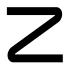
\includegraphics[keepaspectratio]{images/part001_525bb1e1.jpg}}

Note that f is not necessarily uniquely determined by the relation \(u = u' \circ f\) (VIII, p.~170, Exercise 21).

COROLLARY 2. --- Let \((\mathrm{P}, u)\) be a projective cover of the A-module M. If Q is a projective A-module and \(g : Q \to M\) a surjective linear mapping, then there exists a surjective linear mapping \(f : Q \to P\) such that \(g = u \circ f\) .

PROPOSITION 9. --- Let M be an A-module and \((P, u)\) a projective cover of M. Denote the radical of the ring A by r. The homomorphism \(\overline{u}: P/rP \to M/rM\) deduced from u by passing to the quotients is an isomorphism.

The homomorphism \(u\) is surjective by definition, so \(\overline{u}\) is surjective. Denote the kernel of \(u\) by \(N\) . We have \(u^{-1}(\mathfrak{rM}) = N + \mathfrak{rP}\) . Let us prove that we have \(N \subset \mathfrak{rP}\) , which implies the injectivity of \(\overline{u}\) . For every maximal submodule \(P'\) of \(P\) , we have \(u(P') \neq M\) , hence \(P' + N \neq P\) ; since \(P'\) is maximal, we have \(N \subset P'\) . The submodule \(N\) of \(P\) is therefore contained in the radical of \(P\) . Now, the latter is equal to \(\mathfrak{rP}\) by Proposition 6 of VIII, p.~158.

COROLLARY. --- If an A-module M has a projective cover, then the A/r-module M/rM is projective.

Indeed, if \((P,u)\) is a projective cover of M, then the \((A/\mathfrak{r})\) -module M/rM is isomorphic to P/rP (Proposition 9). Since the A-module P is projective, the \((A/\mathfrak{r})\) -module P/rP is also projective.

Remarks. --- 3) Suppose that the ring A is without radical. By Proposition 9, \((P, u)\) is a projective cover of an A-module M if and only if u is an isomorphism. Hence, projective covers can only exist for projective A-modules.

The ring Z is without radical (VIII, p.~154, Example 3). Let \(n \geqslant 2\) be an integer. The Z-module Z/nZ is not projective and therefore does not admit a projective cover.

\begin{enumerate}
\def\labelenumi{\arabic{enumi})}
\setcounter{enumi}{3}
\tightlist
\item
  Suppose that every finitely generated A-module has a projective cover; then the quotient \(A'\) of A by its radical is semisimple. Indeed, every finitely generated module over the ring \(A'\) is projective by the corollary. In particular, for every left ideal \(\mathfrak{a}\) of \(A'\) , the \(A'\) -module \(A_s'/\mathfrak{a}\) is projective. Our assertion then follows from Proposition 4 of VIII, p.~138.
\end{enumerate}

We can give examples of a commutative ring A for which A/r is semisimple and of a finitely generated A-module M that does not admit a projective cover (VIII, p.~170, Exercise 22).

PROPOSITION 10. --- Let M be an A-module, P a projective A-module, and \(u : P \to M\) a linear mapping. Let a be a two-sided ideal of A. Suppose that the linear mapping \(\overline{u} : P / aP \to M / aM\) deduced from u by passing to the quotients is bijective and that one of the following conditions are satisfied:

\begin{enumerate}
\def\labelenumi{(\roman{enumi})}
\item
  The A-modules M and P are finitely generated, and a is contained in the radical of A.
\item
  The ideal \(\mathfrak{a}\) is nilpotent.
\end{enumerate}

Then (P, u) is a projective cover of M.

Under the assumptions, the homomorphism \(u\) is surjective (VIII, p.~159, Corollary 2) and its kernel \(N\) is contained in \(\mathfrak{a}P\) . Let \(P'\) be a proper submodule of \(P\) . By Nakayama's lemma (VIII, p.~158, Theorem 2), we have \(P' + \mathfrak{a}P \neq P\) and therefore \(u(P') \neq M\) . So \((P, u)\) is a projective cover of \(M\) .

COROLLARY 1. --- Let P be a projective A-module. Suppose that P is finitely generated or that the radical r of A is a nilpotent two-sided ideal. Denote the canonical mapping from P to P/rP by u. Then (P, u) is a projective cover of P/rP.

COROLLARY 2. --- Let a be a two-sided ideal of A and M an A-module such that the (A/a)-module M/AM is free. Suppose that one of the following conditions is satisfied:

\begin{enumerate}
\def\labelenumi{(\roman{enumi})}
\item
  The module M is finitely generated, and \(\mathfrak{a}\) is contained in the radical of A.
\item
  The ideal \(\mathfrak{a}\) is nilpotent.
\end{enumerate}

Then M has a projective cover.

More precisely, let P be a free A-module, \((e_{i})_{i\in\mathrm{I}}\) a basis of P, and let \(u:P\to M\) be a homomorphism such that the canonical images of the elements \(u(e_{i})\) of M/aM form a basis of the (A/a)-module M/aM. Then (P,u) is a projective cover of M.

The \((\mathrm{A}/\mathfrak{a})\) -module P/aP is free, and the homomorphism \(\overline{u}\) from P/aP to M/aM deduced from u by passing to the quotients transforms a basis of P/aP into a basis of M/aM, hence is bijective.

If a is nilpotent, then it suffices to apply Proposition 10. Now suppose that the ring A is nonzero and that the module M is finitely generated; then so is the \((A/a)\) -module M/aM, and consequently also the \((A/a)\) -module P/aP. Every basis of P/aP is then finite. It follows that the set I is finite and that the A-module P is finitely generated. We then apply Proposition 10 again.

COROLLARY 3. --- Every finitely generated module over a local ring has a projective cover.

Let A be a local ring and r its radical. It is a two-sided ideal of A (VIII, p.~155, Proposition 5, a)), and the ring A/r is a field (VIII, p.~157, Corollary 4). If M is an A-module, then M/rM is a vector space over the field A/r, hence is a free (A/r)-module. It then suffices to apply Corollary 2.

Remark 5. --- Let A be a local ring and r its radical. Let M be a finitely generated A-module, P a finitely generated projective A-module, and \(u : P \to M\) a homomorphism. By Corollary 6 of VIII, p.~36, the A-module P is free. Choose a basis \((e_{i})_{i \in I}\) of P. Set \(x_{i} = u(e_{i})\) , and denote the canonical image of \(x_{i}\) in M/rM by \(\overline{x}_{i}\) . The following properties are equivalent:

\begin{enumerate}
\def\labelenumi{(\roman{enumi})}
\item
  The pair \((\mathrm{P},u)\) is a projective cover of M.
\item
  The family \((x_{i})_{i\in \mathrm{I}}\) is a minimal generating family of the A-module M.
\item
  The family \((\overline{x}_{i})_{i\in\mathrm{I}}\) is a basis of the vector space M/rM over the field A/r.
\end{enumerate}

We have (i) \(\Rightarrow\) (ii) by Remark 2 of VIII, p.~161 and (iii) \(\Rightarrow\) (i) by Corollary 2. Furthermore, if the family \((x_{i})\) is a minimal generating family of the A-module M, then the family \((\overline{x}_{i})\) is a minimal generating family, that is, a basis, of the vector space M/rM over A/r (VIII, p.~158, Corollary 1).

PROPOSITION 11. --- Let A be a ring and a nilpotent two-sided ideal of A. Let M be a projective A/a-module. There exist a projective A-module P and a surjective A-linear mapping \(u: \mathrm{P} \to \mathrm{M}\) with kernel aP.

Such a pair \((P,u)\) is a projective cover of M viewed as an A-module.

There exists an A/ \(\alpha\) -module \(M'\) such that \(M \oplus M'\) is a free A/ \(\alpha\) -module. Choose a free A-module L and a surjective A-linear mapping \(v: L \to M \oplus M'\) with kernel aL. By Corollary 1 of Proposition 7 (VIII, p.~159), there exists a direct sum decomposition \(L = P \oplus P'\) such that \(v(P) = M\) and \(v(P') = M'\) . The A-module P is projective, and the A-linear mapping u from P to M that coincides with v on P is surjective, with kernel aP. The first assertion follows.

Let P be a projective A-module and u a homomorphism from P to M with kernel aP. By Proposition 10, the pair \((P,u)\) is a projective cover of M.

COROLLARY. --- Let P and P' be projective A-modules. If the modules P/ \(\alpha\) P and P'/ \(\alpha\) P' are isomorphic, then P and P' are isomorphic.

Since P/aP and \(P^{\prime}/aP^{\prime}\) are projective, the corollary follows from Proposition 11 and the uniqueness of the projective cover (VIII, p.~162, Corollary 1).

\BourbakiExercises{Exercises}

\begin{enumerate}
\def\labelenumi{\arabic{enumi})}
\tightlist
\item
  Let \(\mathrm{K}\) be a commutative field of characteristic \(p\) , \(\mathrm{M}\) a \(p\) -primary \(\mathbf{Z}\) -module, \(\mathrm{A}\) the algebra of the group \(\mathrm{M}\) over \(\mathrm{K}\) , and \(\mathfrak{m}\) the set of elements \(\sum_{m} a_{m} e_{m}\) of \(\mathrm{A}\) (cf.~III, §2, No.~6, p.~446) with \(\sum_{m} a_{m} = 0\) .
\end{enumerate}

\begin{enumerate}
\def\labelenumi{\alph{enumi})}
\item
  Prove that A is a local ring, with maximal ideal \(\mathfrak{m}\) , and that \(\mathfrak{m}\) is a nil ideal (cf.~VIII, p.~41, Exercise 10).
\item
  Suppose, moreover, that the homothety \(p_{\mathrm{M}}\) is surjective. Prove that we have \(\mathfrak{m} = \mathfrak{m}^2\) .
\end{enumerate}

\begin{enumerate}
\def\labelenumi{\arabic{enumi})}
\setcounter{enumi}{1}
\item
  Let A be a ring and M an A-module without radical. Prove that the ring of homotheties \(A_{M}\) is without radical (identify \(A_{s}\) with a submodule of \(M^{M}\) ).
\item
  \begin{enumerate}
  \def\labelenumii{\alph{enumii})}
  \tightlist
  \item
    Let A be a ring with semisimple quotient ring \(\mathrm{A} / \Re (\mathrm{A})\) . Prove that we have \(\Re (\mathrm{M}) = \Re (\mathrm{A})\mathrm{M}\) for every A-module M (observe that \(\mathrm{M} / \Re (\mathrm{A})\mathrm{M}\) is an \(\mathrm{A} / \Re (\mathrm{A})\) -module).
  \end{enumerate}
\end{enumerate}

\begin{enumerate}
\def\labelenumi{\alph{enumi})}
\setcounter{enumi}{1}
\tightlist
\item
  Deduce an example of a ring A and a family \((\mathrm{V}_{i})_{i\in\mathrm{I}}\) of A-modules such that \(\Re\big(\prod\mathrm{M}_{i}\big)\neq\prod\Re(\mathrm{M}_{i})\) (use a) for a ring whose radical is not finitely generated).
\end{enumerate}

\begin{enumerate}
\def\labelenumi{\arabic{enumi})}
\setcounter{enumi}{3}
\item
  Let A be an algebra over a commutative field K and a two-sided ideal of A. Let B be the subalgebra of A generated by 1 and a. Prove that the radical of B is contained in that of A (observe that if S is a simple A-module, then we have either ax = 0 for every \(x \in S\) or ax = S for every \(x \neq 0\) in S).
\item
  Let \(A\) be an algebra over a commutative field \(K\) .
\end{enumerate}

\begin{enumerate}
\def\labelenumi{\alph{enumi})}
\tightlist
\item
  Prove that an element of the radical of A that is algebraic over K is nilpotent. b) Suppose that K is an infinite field and that \(\operatorname{Card}(K) > [A : K]\) . Prove that the radical of A is a nil ideal (reason as in Lemma 1 of VIII, p.~47).
\end{enumerate}

\begin{enumerate}
\def\labelenumi{\arabic{enumi})}
\setcounter{enumi}{5}
\tightlist
\item
  Let \(\mathrm{A}\) be a ring.
\end{enumerate}

\begin{enumerate}
\def\labelenumi{\alph{enumi})}
\item
  Let \(\mathfrak{a}\) and \(\mathfrak{b}\) be two-sided ideals of A. If \(\mathfrak{a}\) and \(\mathfrak{b}\) are nilpotent (resp. nil ideals), then so is \(\mathfrak{a} + \mathfrak{b}\) .
\item
  Prove that the sum \(\mathfrak{G}\) of all two-sided nil ideals is a two-sided nil ideal and that the sum \(\mathfrak{N}\) of all nilpotent two-sided ideals is a two-sided nil ideal that contains all nilpotent ideals (VIII, p.~149, Exercise 3).
\item
  Prove that G is the largest semiprime nil ideal (loc. cit.) of A; we say that G is the nilradical of A. If A is commutative, then G and N are both equal to the set of nilpotent elements of A.
\end{enumerate}

¶ 7) Let A be a ring, and let I be the set of ordinals \(\alpha\) such that \(\text{Card}(\alpha) \leqslant \text{Card}(A)\) (Set Theory, III, §6, p.~241, Exercise 10). Define two-sided ideals \(\mathfrak{N}_{\alpha}\) for all \(\alpha \in I\) as follows by transfinite induction. Take \(\mathfrak{N}_0 = \mathfrak{N}\) (Exercise 6, b)). If \(\alpha\) admits a successor \(\alpha + 1\) , then \(\mathfrak{N}_{\alpha+1}\) is the two-sided ideal such that \(\mathfrak{N}_{\alpha+1}/\mathfrak{N}_{\alpha}\) is the sum of the nilpotent two-sided ideals of \(A/\mathfrak{N}_{\alpha}\) . If \(\alpha\) is a limit ordinal, take \(\mathfrak{N}_{\alpha}\) to be the union of the \(N_{\beta}\) for \(\beta < \alpha\) . Let \(\tau\) be the smallest ordinal such that \(N_{\tau+1} = N_{\tau}\) ; the ideal \(P = N_{\tau}\) is called the prime radical of A.

\begin{enumerate}
\def\labelenumi{\alph{enumi})}
\item
  Prove that we have \(N \subset P \subset G\) and that P is the smallest semiprime nil ideal of A. \(^{(1)}\)
\item
  Prove that \(\mathfrak{P}\) is the intersection of the semiprime two-sided ideals of A (cf.~VIII, p.~149, Exercise 3).
\item
  Prove that P is the intersection of the prime two-sided ideals of A (loc. cit., c)). d) Prove that P is the set of elements a of A with the following property: every sequence \((a_{n})_{n\geqslant0}\) of elements of A such that \(a_{0}=a\) and \(a_{n+1}\in a_{n}Aa_{n}\) for every n has finite support (same method as in loc. cit.).
\end{enumerate}

\begin{enumerate}
\def\labelenumi{\arabic{enumi})}
\setcounter{enumi}{7}
\tightlist
\item
  We keep the notation of Exercise 7. Let A be a left Noetherian ring.
\end{enumerate}

\begin{enumerate}
\def\labelenumi{\alph{enumi})}
\item
  Prove that \(\mathfrak{N}\) is the largest nilpotent two-sided ideal of A and that it is equal to the prime radical \(\mathfrak{P}\) of A.
\item
  Prove that every left or right nil ideal of A is nilpotent (apply Exercise 5, a) of VIII, p.~150 to the ring A/N). We therefore have \(\mathfrak{N} = \mathfrak{P} = \mathfrak{G}\) .
\end{enumerate}

\begin{enumerate}
\def\labelenumi{\arabic{enumi})}
\setcounter{enumi}{8}
\item
  Let \(\mathrm{K}\) be a commutative field, \(\mathrm{B}\) the ring \(\mathrm{K}[(\mathrm{X}_n)_{n\geqslant 1}]\) , \(\mathfrak{I}\) the ideal of \(\mathrm{B}\) generated by the sequence \((\mathrm{X}_n^n)\) , and \(\mathrm{A}\) the ring \(\mathrm{B} / \mathfrak{I}\) . Prove that the radical of \(\mathrm{A}\) is a nil ideal but is not nilpotent.
\item
  Let A be a ring.
\end{enumerate}

\begin{enumerate}
\def\labelenumi{\alph{enumi})}
\item
  Let Z be the center of A. Prove that we have \(Z \cap \Re(A) \subset \Re(Z)\) (cf.~Exercise 15, b) below for an example where the inclusion is strict).
\item
  Prove that \(\Re(\mathrm{A})\) contains no nonzero idempotents.
\item
  Prove that the intersection of \(\Re(\mathrm{A})\) and the left socle s of A (VIII, p.~130, Exercise 8) is a two-sided ideal with square zero and that it is the intersection of s and its left annihilator (use Exercises 7 and 8, a) of VIII, p.~130).
\end{enumerate}

\(d\) ) Let \(e\) be an idempotent in A. Prove that the radical of the ring \(e\mathrm{A}e\) is \(e\Re (\mathrm{A})e\) (observe that for \(a\in e\mathrm{A}e\) , we have \((1 - a)(1 - e) = (1 - e)(1 - a) = 1 - e\) ).

\begin{enumerate}
\def\labelenumi{\alph{enumi})}
\setcounter{enumi}{4}
\tightlist
\item
  Prove that the radical of the ring \(\mathbf{M}_{n}(\mathrm{A})\) is the ideal \(\mathbf{M}_{n}(\Re(\mathrm{A}))\) (VIII, p.~114, Example 2).
\end{enumerate}

\begin{enumerate}
\def\labelenumi{\arabic{enumi})}
\setcounter{enumi}{10}
\tightlist
\item
  Let A be a commutative ring and B the ring A{[}X{]}.
\end{enumerate}

\begin{enumerate}
\def\labelenumi{\alph{enumi})}
\item
  First, assume that A has no nonzero nilpotent elements. Let \(f = \sum_{i} a_{i} X^{i}\) and \(g = \sum_{i} b_{i} X^{i}\) be two elements of B. Prove that we have \(a_{p} b_{q} = 0\) for \(p + q > \deg(fg)\) . b) Let N be the nilradical of A (Exercise 6). Prove that a polynomial \(f \in B\) is invertible in B if and only if its constant term is invertible in A and its other coefficients belong to N (apply a) to the image of f in \((\mathrm{A}/\mathfrak{N})[\mathrm{X}]\) .
\item
  Deduce that the radical of B is the ideal \(\Re[X]\) and that it is equal to the nilradical of B.
\end{enumerate}

\begin{enumerate}
\def\labelenumi{\arabic{enumi})}
\setcounter{enumi}{11}
\tightlist
\item
  \begin{enumerate}
  \def\labelenumii{\alph{enumii})}
  \tightlist
  \item
    A ring A is without radical if and only if it is isomorphic to a subring C of a product \(\prod_{i\in I}B_{i}\) of primitive rings such that \(\mathrm{pr}_{i}(\mathrm{C})=\mathrm{B}_{i}\) for every \(i\in I\) (consider the set of classes of simple A-modules).
  \end{enumerate}
\end{enumerate}

\begin{enumerate}
\def\labelenumi{\alph{enumi})}
\setcounter{enumi}{1}
\tightlist
\item
  Let V be an infinite-dimensional vector space over a field D, let B be the ring \(\operatorname{End}_{\mathrm{D}}(\mathrm{V})\) , and let s be its socle (cf.~VIII, p.~130, Exercise 8). Let C be the subring of \(B \times B\) generated by \(s \times s\) and the unit element. Prove that C is without radical but is not isomorphic to a product of primitive rings.
\end{enumerate}

\begin{enumerate}
\def\labelenumi{\arabic{enumi})}
\setcounter{enumi}{12}
\item
  Let \(G\) be a commutative group without torsion and \(K\) a commutative field. Prove that the algebra \(K[G]\) is without radical (endow \(G\) with a total ordering compatible with its group structure, cf.~VI, §1, p.~32, Exercise 20).
\item
  Let \(\mathrm{K}\) be an ordered commutative field and \(\mathrm{G}\) a group. Prove that the algebra of the group \(\mathrm{G}\) over \(\mathrm{K}\) does not admit a nonzero (left or right) nil ideal. (For \(x = \sum a_{g}e_{g}\) , set \(t(x) = a_{1}\) and \(x^{*} = \sum a_{g}e_{g - 1}\) . Observe that if \(x\) is nonzero, then we have \(t((xx^{*})^{2k}) > 0\) for every \(k\geqslant 0\) .) Prove the same property for the algebra of \(\mathrm{G}\) over the field \(\mathrm{K}(i)\) , where \(i^2 = -1\) .
\item
  Let \(V_{0}\) be a vector space of finite dimension n over a field D, and let B be a subring of the ring \(\operatorname{End}_{\mathrm{D}}(\mathrm{V}_{0})\) . Set \(V_{k}=V_{0}\) for \(k\geqslant1\) and \(V=\oplus_{k\geqslant0}V_{k}\) . Consider the set A of endomorphisms u of V for which there exists an integer m (that depends on u) such that we have \(u(V_{k})\subset\oplus_{i\leqslant m}V_{i}\) for \(k\leqslant m\) and \(u(V_{k})\subset V_{k}\) for k\textgreater m and that for k\textgreater m, the endomorphism of \(V_{k}\) obtained by restriction is independent of k and belongs to B.
\end{enumerate}

\begin{enumerate}
\def\labelenumi{\alph{enumi})}
\tightlist
\item
  Prove that A is a primitive ring and that its socle consists of the elements u of A such that \(u(\mathrm{V}_{k}) = 0\) for all but finitely many indices k (VIII, p.~130, Exercise 8).
\item
  Choose suitable D, n, and B to give an example of a primitive ring that has a quotient ring with nilpotent nonzero radical and an example of a primitive ring whose center has nonzero radical.
\end{enumerate}

\begin{enumerate}
\def\labelenumi{\arabic{enumi})}
\setcounter{enumi}{15}
\tightlist
\item
  Let A be a ring and \(\mathfrak{a}\) a two-sided ideal contained in the radical of A. Let M and N be A-modules and \(u: \mathrm{M} \to \mathrm{N}\) a homomorphism. We denote by \(\overline{u}: \mathrm{M} / \mathfrak{aM} \to \mathrm{N} / \mathfrak{aN}\) the homomorphism of A/ \(\mathfrak{a}\) -modules deduced from \(u\) .
\end{enumerate}

\begin{enumerate}
\def\labelenumi{\alph{enumi})}
\item
  Suppose that M and N are finitely generated and N is projective. If \(\overline{u}\) is bijective, then so is u.
\item
  Give an example with M and N free of rank 1 and \(\overline{u}\) injective but \(\operatorname{Ker}(u) \neq 0\) . c) Suppose that M and N are projective. If \(\overline{u}\) induces an isomorphism to a direct factor, then u is injective (reduce to the case when M and N are free and equal and \(\overline{u}\) is the identity, and then use a)). If, moreover, M is finitely generated, then the image of u is a direct factor of N.
\item
  Suppose that M is finitely generated and N is projective. If \(\overline{u}\) is bijective, then so is u (apply c) to a homomorphism \(v: N \to M\) such that \(\overline{v} = \overline{u}^{-1}\) to conclude that N is finitely generated).
\item
  If M is projective and M/ \(\mathfrak{aM}\) is zero, then M is zero.
\end{enumerate}

\begin{enumerate}
\def\labelenumi{\arabic{enumi})}
\setcounter{enumi}{16}
\tightlist
\item
  Let \(\mathbf{K}\) be a commutative field and \(\mathbf{L}\) a set.
\end{enumerate}

\begin{enumerate}
\def\labelenumi{\alph{enumi})}
\tightlist
\item
  Prove that there exists a K-algebra A admitting a basis consisting of the unit element, a family \((c_{\lambda})_{\lambda \in \mathrm{L}}\) , and a family \((r_{\lambda \mu})_{(\lambda ,\mu)\in \mathrm{L}\times \mathrm{L}}\) , with multiplication table
\end{enumerate}

\[
\begin{array}{r} c _ {\lambda} ^ {2} = c _ {\lambda}, \qquad c _ {\lambda} c _ {\mu} = r _ {\lambda \mu} \quad \mathrm{if} \lambda \neq \mu \\ c _ {\lambda} r _ {\mu \nu} = \delta_ {\lambda \mu} r _ {\mu \nu}, \qquad r _ {\lambda \mu} c _ {\nu} = \delta_ {\mu \nu} r _ {\lambda \mu} \\ r _ {\lambda \mu} r _ {\nu \rho} = 0, \end{array}
\]

where \(\delta_{\mu\nu}\) is the Kronecker delta function. Prove that \(\Re(\mathrm{A})\) is the subalgebra of A generated by the \(r_{\lambda\mu}\) ; we have \(\Re(\mathrm{A})^{2}=0\) .

\begin{enumerate}
\def\labelenumi{\alph{enumi})}
\setcounter{enumi}{1}
\tightlist
\item
  Suppose \(\operatorname{Card}(\mathrm{L}) \geqslant 2\) . Prove that the center Z of A is the K-vector space generated by 1, the \(r_{\lambda\lambda}\) for \(\lambda \in L\) , and, if L is finite, the element \(\sum_{\lambda} c_{\lambda} - \sum_{\mu \neq \nu} r_{\mu\nu}\) . Deduce that for \(\lambda \in L\) , there are no idempotents in Z congruent to \(c_{\lambda} \pmod{\Re(A)}\) .
\end{enumerate}

¶ 18) a) Let A be a ring, a a two-sided nil ideal of A, and \((\overline{e}_{n})_{n\geqslant1}\) an orthogonal sequence of idempotents in A/a. Prove that there exists an orthogonal sequence \((e_{n})_{n\geqslant1}\) of idempotents in A such that \(\overline{e}_{n}\) is the class of \(e_{n}\) in A/a for every n.~(Let \(\overline{e}\) and \(\overline{e}'\) be two orthogonal idempotents in A/a, \(e'\) an idempotent in A lifting \(\overline{e}'\) , and let a be a representative of e in A. Observe that we can modify a to have \(ae' = e'a\) , and then, as in Proposition 7 of VIII, p.~159, to have \(a^{2} = a\) .)

\begin{enumerate}
\def\labelenumi{\alph{enumi})}
\setcounter{enumi}{1}
\tightlist
\item
  Let K be a commutative field, L an uncountable set, and A the K-algebra defined in the previous exercise. Prove that there does not exist any orthogonal family \((e_{\lambda})_{\lambda\in\mathrm{L}}\) of idempotents in A satisfying \(e_{\lambda}\equiv c_{\lambda} \pmod{\Re(\mathrm{A})}\) for every \(\lambda\in L\) . (Consider the set H of elements \((\lambda,\mu)\) of \(L\times L\) such that \(c_{\lambda}(e_{\mu}-c_{\mu})=0\) . Observe that the sets \(H\cap(\{\lambda\}\times L)\) are finite for every \(\lambda\in L\) and the sets \(\mathbb{C}H\cap(L\times\{\mu\})\) are finite for every \(\mu\in L\) .)
\end{enumerate}

\begin{enumerate}
\def\labelenumi{\arabic{enumi})}
\setcounter{enumi}{18}
\item
  Let A be a ring, a a two-sided ideal of A contained in \(\Re(\mathrm{A})\) , let e and \(e'\) be idempotents in A, and let \(\overline{e}\) and \(\overline{e}'\) their classes in the ring \(\overline{A} = A/a\) . Prove that if the idempotents \(\overline{e}\) and \(\overline{e}'\) are equivalent (VIII, p.~39, Exercise 5), then so are e and \(e'\) (observe that Ae is a projective cover of the A-module \(\overline{A}\overline{e}\) ).
\item
  Let \(\mathrm{A}\) be an algebra over a commutative field \(\mathrm{K}\) such that \(\Re(\mathrm{A})\) is a nil ideal and that the algebra \(\mathrm{A} / \Re(\mathrm{A})\) is isomorphic to a finite product of matrix algebras over \(\mathrm{K}\) . Prove that there exists a subalgebra \(\mathrm{S}\) of \(\mathrm{A}\) such that the \(\mathrm{K}\) -vector space \(\mathrm{A}\) is the direct sum of \(\mathrm{S}\) and \(\Re(\mathrm{A})\) (use Exercises 18 and 19 above, as well as Exercise 19 of VIII, p.~94).
\item
  Let A be a ring, \(u: P \to M\) a surjective homomorphism of A-modules, and N its kernel. We denote by \(\operatorname{End}_{\mathrm{A}}(\mathrm{P}; \mathrm{N})\) (resp. \(\operatorname{Aut}_{\mathrm{A}}(\mathrm{P}; \mathrm{N})\) ) the ring of endomorphisms (resp. the group of automorphisms) u of P such that \(u(\mathrm{N}) \subset \mathrm{N}\) .
\end{enumerate}

\begin{enumerate}
\def\labelenumi{\alph{enumi})}
\tightlist
\item
  Define an exact sequence
\end{enumerate}

\[
0 \to \mathrm{Hom} _ {\mathrm{A}} (\mathrm{P}, \mathrm{N}) \xrightarrow {i} \mathrm{End} _ {\mathrm{A}} (\mathrm{P}; \mathrm{N}) \xrightarrow {p} \mathrm{End} _ {\mathrm{A}} (\mathrm{M})
\]

where the image of \(i\) is a two-sided ideal \(\mathfrak{I}\) of the ring \(\operatorname{End}_{\mathrm{A}}(\mathrm{P};\mathrm{N})\) .

\begin{enumerate}
\def\labelenumi{\alph{enumi})}
\setcounter{enumi}{1}
\tightlist
\item
  Suppose that \((P, u)\) is a projective cover of M. Then p is surjective and induces a surjective homomorphism \(p' : \operatorname{Aut}_{\mathrm{A}}(\mathrm{P}; \mathrm{N}) \to \operatorname{Aut}_{\mathrm{A}}(\mathrm{M})\) . We have an exact sequence of groups
\end{enumerate}

\[
0 \to 1 _ {\mathrm{P}} + \Im \to \mathrm{Aut} _ {\mathrm{A}} (\mathrm{P}; \mathrm{N}) \xrightarrow {p ^ {\prime}} \mathrm{Aut} _ {\mathrm{A}} (\mathrm{M}) \to 0;
\]

if P is free and N is not reduced to 0, then the homomorphism \(p'\) is not injective.

\begin{enumerate}
\def\labelenumi{\arabic{enumi})}
\setcounter{enumi}{21}
\tightlist
\item
  Let \(A\) be a commutative integral domain that has only a finite number \(s > 1\) of maximal ideals \(\mathfrak{m}_1, \ldots, \mathfrak{m}_s\) .
\end{enumerate}

\begin{enumerate}
\def\labelenumi{\alph{enumi})}
\item
  Prove that the ring A/ \(\Re(A)\) is isomorphic to the product of the fields A/mi.
\item
  Prove that the A-modules \(A/m_{i}\) do not admit a projective cover even though they are projective and finitely generated as \(A/\Re(A)\) -modules (observe that A is a projective cover of \(A/\Re(A)\) ).
\item
  Let K be a commutative field. Prove that the subring A of the field \(\mathrm{K(T)}\) consisting of the rational fractions that can be written as \(\mathrm{P(T)/Q(T)}\) with \(\mathrm{Q(0) \neq 0}\) and \(\mathrm{Q(1) \neq 0}\) has the required properties.
\end{enumerate}

\begin{enumerate}
\def\labelenumi{\arabic{enumi})}
\setcounter{enumi}{22}
\item
  Let A be a ring and a a (left) ideal of A. Suppose that for every sequence \((a_{n})_{n\geqslant1}\) of elements of a, there exists an integer m such that \(a_{1}\cdots a_{m}=0\) . Prove that we have \(aM\neq M\) for every nonzero A-module M (if not, construct, by induction, sequences \((a_{n})_{n\geqslant1}\) in a and \((x_{n})_{n\geqslant1}\) in M such that we have \(a_{1}\cdots a_{p}x_{p}\neq0\) for every p).
\item
  Let \(A\) be a ring and \(\mathfrak{r}\) its radical. Prove that the following properties are equivalent:
\end{enumerate}

\begin{enumerate}
\def\labelenumi{(\roman{enumi})}
\tightlist
\item
  Every finitely generated left A-module admits a projective cover.
\end{enumerate}

(i') Every finitely generated right A-module admits a projective cover.

\begin{enumerate}
\def\labelenumi{(\roman{enumi})}
\setcounter{enumi}{1}
\tightlist
\item
  The ring \(\mathrm{A} / \mathfrak{r}\) is semisimple, and every idempotent in \(\mathrm{A} / \mathfrak{r}\) is the class of an idempotent in \(\mathrm{A}\) .
\end{enumerate}

(To prove (i)⇒(ii), observe that every decomposition \(A/r = a_{1} \oplus a_{2}\) into a direct sum of ideals lifts to a decomposition \(A = P_{1} \oplus P_{2}\) , where \(P_{i}\) is a projective cover of \(a_{i}\) . Show that, moreover, (ii) implies that every A/r-module is of the form \((\mathrm{A}/\mathfrak{r}) \otimes_{\mathrm{A}} \mathrm{P}\) , where P is a projective A-module.)

¶ 25) Let A be a ring and r its radical. Prove that the following conditions are equivalent:

\begin{enumerate}
\def\labelenumi{(\roman{enumi})}
\tightlist
\item
  Every left A-module admits a projective cover.
\end{enumerate}

(i') Every right A-module admits a projective cover.

\begin{enumerate}
\def\labelenumi{(\roman{enumi})}
\setcounter{enumi}{1}
\tightlist
\item
  The ring A/r is semisimple, and for every sequence \((a_{n})_{n\geqslant1}\) of elements of r, there exists an integer m such that \(a_{1}\cdots a_{m}=0\) .
\end{enumerate}

(Prove (ii)⇒(i) in the same way as the corresponding implication of Exercise 24, using Exercise 23. Assume that condition (i) is satisfied. Consider the submodule M of A \(^{(N)}\) generated by \(e_1 - a_1e_2\) , \(e_2 - a_2e_3\) , \ldots{} Deduce from Exercise 16, e) applied to a projective cover of A \(^{(N)}\) /M that we have M = A \(^{(N)}\) , which implies that \(a_1 \cdots a_n = 0\) for n sufficiently large.)

\begin{enumerate}
\def\labelenumi{\arabic{enumi})}
\setcounter{enumi}{25}
\tightlist
\item
  A ring A is called a Zorn ring if every left ideal of A that is not a nil ideal contains a nonzero idempotent.
\end{enumerate}

\begin{enumerate}
\def\labelenumi{\alph{enumi})}
\item
  Prove that in a Zorn ring, every right ideal that is not a nil ideal contains a nonzero idempotent (observe that for every nonnilpotent element \(a\) of A, there exists an \(x \in A\) such that \(xaxa = xa \neq 0\) ).
\item
  Prove that the radical of a Zorn ring is a nil ideal and that a Zorn ring without zero divisors is a field.
\item
  Prove that a primitive ring with nonzero socle is a Zorn ring (cf.~VIII, p.~129, Exercise 4, b) and p.~130, Exercise 7, a)). Give an example of a primitive ring that is not a Zorn ring (cf.~VIII, p.~132, Exercise 13) and an example of a primitive ring whose socle is nonzero but whose center is not a Zorn ring (use the method of Exercise 12).
\end{enumerate}

\(d\) ) Let K be a commutative field and A the subring of \(\mathrm{K}(\mathrm{X})^{\mathbf{N}}\) consisting of the sequences \(s = (f_n)\) for which there exists a polynomial \(\varphi(s) \in \mathrm{K}[\mathrm{X}]\) such that \(f_n\) is equal to \(\varphi(s)\) for \(n\) sufficiently large. Prove that A is a commutative Zorn ring, without radical, containing elements that are neither invertible nor zero divisors, but that its image \(\varphi(A)\) is not a Zorn ring.

¶ 27) A ring A is called absolutely flat, or von Neumann regular, if for every element a of A, there exists an \(x \in A\) such that axa = a.

\begin{enumerate}
\def\labelenumi{\alph{enumi})}
\item
  A ring A is absolutely flat if and only if every monogenous left (or right) ideal of A admits a supplement in \(A_{s}\) (that is, is generated by an idempotent).
\item
  Show that every finitely generated ideal of an absolutely flat ring is generated by an idempotent. (Reduce to the case of an ideal \(Ae + Af\) , where e and f are idempotents. Then, by replacing Ae with \(Ae(1 - f)\) , reduce to the case when ef = 0, and consider the element \(e + f - fe\) .) A (left or right) Noetherian absolutely flat ring is semisimple.
\item
  Deduce from b) that the intersection of two monogenous left (resp. right) ideals of an absolutely flat ring is monogenous (consider the right annihilators).
\item
  Every quotient ring of an absolutely flat ring is absolutely flat, as is every product of absolutely flat rings.
\item
  Prove that the radical of an absolutely flat ring is reduced to 0. Deduce that every two-sided ideal of A is the intersection of the maximal left ideals containing it.
\end{enumerate}

\(f\) ) The center of an absolutely flat ring is absolutely flat (prove that if \(a \in \mathbb{Z}\) and \(x \in \mathrm{A}\) satisfy \(a^2 x = a\) , then we have \(a^2 x^n \in \mathbb{Z}\) for every \(n \geqslant 0\) and \(a(a^2 x^3)a = a\) ). \(g\) ) Prove that the endomorphism ring of a vector space is an absolutely flat ring.

¶ 28) Let A be an absolutely flat ring (Exercise 27) and n an integer.

\begin{enumerate}
\def\labelenumi{\alph{enumi})}
\item
  Prove that every finitely generated submodule of \(A^{n}\) admits a supplementary submodule. (Reason by induction on n, by showing that \(M \cap A^{n-1}\) is finitely generated and choosing supplementary submodules of \(M \cap A^{n-1}\) in \(A^{n-1}\) and of the image of M in \(Ae_{n}\) .)
\item
  Deduce that the ring \(\mathbf{M}_n(\mathrm{A})\) is absolutely flat (cf.~VIII, p.~114, Example 2).
\end{enumerate}

\begin{enumerate}
\def\labelenumi{\arabic{enumi})}
\setcounter{enumi}{28}
\item
  Let V be a vector space of countable dimension over a commutative field K, and let \(A = \text{End}_{\text{K}}(\text{V})\) . Prove that there exists a unique maximal two-sided ideal that is \(\text{End}_{\text{K}}^{\text{f}}(\text{V})\) , the set of endomorphisms of finite rank (cf.~Exercise 2 of VIII, p.~128), but that the radical of A is 0.
\item
  \begin{enumerate}
  \def\labelenumii{\alph{enumii})}
  \tightlist
  \item
    Let A be a ring that contains no nilpotent elements other than 0. Prove that every idempotent e in A belongs to the center of A (consider the elements \((1-e)xe\) and \(ex(1-e)\) ).
  \end{enumerate}
\end{enumerate}

\begin{enumerate}
\def\labelenumi{\alph{enumi})}
\setcounter{enumi}{1}
\item
  Let A be an absolutely flat ring that contains no nilpotent elements other than 0, and let a be a nonzero element of A. Prove that there exists an element x of A such that e = ax = xa is idempotent and ea = ae = a. Deduce that for every \(y \in A\) , there exists a \(z \in A\) such that ya = az and, consequently, that every left or right ideal of A is two-sided.
\item
  Prove that no quotient ring of A contains a nonzero nilpotent element (use b)). Deduce that A is isomorphic to a subring C of a product \(\prod_{\iota\in I}D_{\iota}\) of fields such that \(\mathrm{pr}_{\iota}(\mathrm{C})=\mathrm{D}_{\iota}\) for every \(\iota\in I\) (deduce from b) and Exercise 4 of VIII, p.~129 that an absolutely flat primitive ring without nilpotent elements is a field, and use Exercise 12 above).
\end{enumerate}

\(d\) ) Let \((\mathrm{D}_{\iota})_{\iota \in \mathbb{I}}\) be an infinite family of fields and B the ring \(\prod_{\iota \in \mathrm{I}}\mathrm{D}_{\iota}\) . For any subset H of I, denote by \(\mathrm{B_H}\) the two-sided ideal of B consisting of the families \((b_{\iota})_{\iota \in \mathrm{I}}\) such that \(b_{\iota} = 0\) for \(\iota \notin \mathrm{H}\) . Let \(\mathfrak{F}\) be an increasing directed set of subsets of I forming a cover of I, and let A be the subring of B generated by 1 and the \(\mathrm{B_H}\) for \(\mathrm{H}\in \mathfrak{F}\) . Prove that A is absolutely flat and contains no nonzero nilpotent elements.

\begin{enumerate}
\def\labelenumi{\arabic{enumi})}
\setcounter{enumi}{30}
\tightlist
\item
  Let K be a commutative field, and let A be the set of matrices of the form \(\begin{pmatrix} a & b \\ 0 & c \end{pmatrix}\) with \(a, b, c \in K\) . Verify that A is a subring of the matrix ring and that its radical is determined by a = c = 0. Prove that the image of \(\begin{pmatrix} 1 & 0 \\ 0 & 0 \end{pmatrix}\) in A/Re(A) is an idempotent element of the center of A/Re(A).
\end{enumerate}

\section{Modules over an Artinian Ring}

\subsection{The Radical of an Artinian Ring}

PROPOSITION 1. --- Let A be a left Artinian ring. The radical r of A is the largest nilpotent two-sided ideal of A, and the ring A/r is semisimple.

We know (VIII, p.~156, Theorem 1) that every nilpotent two-sided ideal of A is contained in r. Let us prove that r is nilpotent. Since the ring A is left Artinian and the sequence of two-sided ideals \(r^{n}\) is decreasing, there exists an integer \(p \geqslant 0\) such that we have \(r^{p} = r^{p+1}\) . Since A is Artinian, the A-module \(A_{s}\) has finite length (VIII, p.~6, Theorem 1) and is therefore Noetherian. The left ideal \(r^{p}\) is therefore finitely generated. By Nakayama's lemma (Theorem 2 of VIII, p.~158), it follows that \(r^{p} = 0\) .

The ring A/r is without radical (VIII, p.~155, Proposition 5); since it is left Artinian, it is semisimple (VIII, p.~154, Proposition 4).

COROLLARY 1. --- A ring is semisimple if and only if it is left Artinian and has no nilpotent two-sided ideals other than 0.

A semisimple ring is left Artinian and without radical (VIII, p.~154, Proposition 4); it therefore has no nilpotent two-sided ideals other than 0. The converse follows from Proposition 1.

COROLLARY 2. --- In a left Artinian ring A, the radical consists of the elements x such that ax is nilpotent for every a in A.

If A is left Artinian, then the radical is a nilpotent two-sided ideal (Proposition 1). Every left nil ideal is contained in the radical by Jacobson's theorem (VIII, p.~156, Theorem 1). Corollary 2 follows.

\subsection{Modules over an Artinian Ring}

PROPOSITION 2. --- Let A be a left Artinian ring. For every A-module M, the following properties are equivalent:

\begin{enumerate}
\def\labelenumi{(\roman{enumi})}
\item
  M is semisimple.
\item
  M is without radical.
\item
  M is annihilated by the radical r of A.
\end{enumerate}

We know that (i) implies (ii) (VIII, p.~153, Proposition 3). On the other hand, rM is contained in the radical of M (VIII, p.~158, Proposition 6), so (ii) implies (iii).

Suppose that the A-module M is annihilated by r. We can view it as a module over the ring A/r. Now, the ring A/r is semisimple (VIII, p.~173, Proposition 1), and every module over a semisimple ring is semisimple (VIII, p.~138, Proposition 4). Consequently, M is a semisimple module over the ring A/r and a fortiori over the ring A. Hence (iii) implies (i).

COROLLARY. --- Let A be a left Artinian ring. For every A-module M, the radical of M is equal to rM.

The radical \(\Re(\mathrm{M})\) of M contains rM (VIII, p.~158, Proposition 6). Moreover, the A-module M/rM is annihilated by r. By Proposition 2, it is therefore without radical, which implies \(\Re(\mathrm{M}) \subset \mathfrak{rM}\) (VIII, p.~152, Corollary 1, c)).

PROPOSITION 3. --- Let A and B be rings and f a homomorphism from A to B such that B is generated by the union of \(f(\mathrm{A})\) and the commutant \(f(\mathrm{A})'\) of \(f(\mathrm{A})\) in B. Let M be a left B-module. Suppose that either the ring A is left Artinian or the A-module \(f_{*}(\mathrm{M})\) deduced from M by restriction of scalars (II, §1, No.~13, p.~221) is finitely generated. We then have \(\mathfrak{R}_{\mathrm{A}}(f_{*}(\mathrm{M})) \subset \mathfrak{R}_{\mathrm{B}}(\mathrm{M})\) .

Let S be a simple B-module. Suppose that either A is left Artinian or the A-module \(f_{*}(S)\) is finitely generated. We will prove that \(f_{*}(S)\) is without radical. For every \(b \in f(A)'\) , the homothety \(b_{S}\) is an endomorphism of the A-module \(f_{*}(S)\) and therefore preserves \(\mathfrak{R}_{\mathrm{A}}(f_{*}(\mathrm{S}))\) (VIII, p.~152, Proposition 1). Since B is generated by \(f(\mathrm{A}) \cup f(\mathrm{A}')\) , the radical \(\mathfrak{R}_{\mathrm{A}}(f_{*}(\mathrm{S}))\) is a B-submodule of S, hence equal to 0 or S. If \(f_{*}(S)\) is a finitely generated A-module, then we have \(\mathfrak{R}_{\mathrm{A}}(f_{*}(\mathrm{S})) \neq f_{*}(\mathrm{S})\) (VIII, p.~153, Proposition 2). If the ring A is left Artinian, then we have \(\mathfrak{R}_{\mathrm{A}}(f_{*}(\mathrm{S})) = f(\mathfrak{r})\mathrm{S}\) , where r is the radical of A (VIII, p.~174, Corollary of Proposition 2), and since r is a nilpotent two-sided ideal of A (VIII, p.~173, Proposition 1), we cannot have \(S = f(\mathfrak{r})S\) . We therefore have \(\mathfrak{R}_{\mathrm{A}}(f_{*}(\mathrm{S})) = 0\) in both cases.

Let u be a nonzero B-linear mapping from M to a simple M-module S. The mapping u is surjective; consequently, if \(f_{*}(\mathrm{M})\) is finitely generated, then so is \(f_{*}(\mathrm{S})\) . Under the assumptions of Proposition 3, the A-module \(f_{*}(\mathrm{S})\) is without radical and u is an A-linear mapping from \(f_{*}(\mathrm{M})\) to \(f_{*}(\mathrm{S})\) . Hence, the kernel of u contains \(\mathfrak{R}_{\mathrm{A}}(f_{*}(\mathrm{M}))\) by Proposition 1 of VIII, p.~152. Since u is arbitrary, we have \(\mathfrak{R}_{\mathrm{A}}(f_{*}(\mathrm{M})) \subset \mathfrak{R}_{\mathrm{B}}(\mathrm{M})\) .

COROLLARY. --- Let A be a commutative ring and B an algebra over A. Suppose that either the ring A is Artinian or B is a finitely generated A-module. We then have \(\Re(\mathrm{A})\mathrm{B}\subset\Re(\mathrm{B})\) .

By Proposition 3, the radical \(\mathfrak{R}_{\mathrm{A}}(\mathrm{B}_{s})\) is contained in \(\mathfrak{R}_{\mathrm{B}}(\mathrm{B}_{s})\) , which is nothing but the radical of the ring B. Moreover, we have \(\mathfrak{R}(\mathrm{A})\mathrm{B}\subset\mathfrak{R}_{\mathrm{A}}(\mathrm{B}_{s})\) by Proposition 6 of VIII, p.~158. The corollary follows.

\subsection{Projective Modules over an Artinian Ring}

PROPOSITION 4. --- Every module over a left Artinian ring has a projective cover.

Let A be a left Artinian ring, and let M be a module over A. The radical r of A is a nilpotent two-sided ideal, and the ring A/r is semisimple (VIII, p.~173, Proposition 1). It follows that the A/r-module M/rM is projective. The assertion then follows from Proposition 11 of VIII, p.~164.

PROPOSITION 5. --- Let A be a left Artinian ring and r its radical.

\begin{enumerate}
\def\labelenumi{\alph{enumi})}
\item
  Let P be a projective A-module. Denote the canonical mapping from P to P/rP by u. Then \((P,u)\) is a projective cover of P/rP. In particular, the A-module P is finitely generated if and only if P/rP is.
\item
  Let M be a module over the ring A/r. Then M, viewed as an A-module, has a projective cover. If \((P,u)\) is such a projective cover, then when passing to the quotient, u induces an isomorphism from P/rP to M. Moreover, P is indecomposable if and only if M is simple.
\item
  Let M and M' be modules over the ring A/r. Let \((P, u)\) and \((P', u')\) be projective covers of the A-modules M and M'. Then M and M' are isomorphic if and only if P and P' are.
\end{enumerate}

The radical r of A is a nilpotent two-sided ideal (VIII, p.~173, Proposition 1). Assertion a) therefore follows from Corollary 1 of VIII, p.~163 and Remark 2 of VIII, p.~161.

Let us prove assertion b). The existence of a projective cover \((P, u)\) of M follows from Proposition 4 and the isomorphism from P/rP to M of Proposition 9 of VIII, p.~162. Since the ring A/r is semisimple, a module over this ring is indecomposable if and only if it is simple. The last assertion then follows from Corollary 2 of VIII, p.~160.

Let us prove c). Let f be an isomorphism from P to \(P'\) ; it induces an isomorphism \(\overline{f}\) from \(P/rP\) to \(P'/rP'\) . By b), these quotients are isomorphic to M and \(M'\) , respectively. Therefore, M is isomorphic to \(M'\) . Conversely, by Proposition 8 of VIII, p.~161, every isomorphism f from M to \(M'\) lifts to an isomorphism \(\widetilde{f}\) from P to \(P'\) such that \(f \circ u = u' \circ \widetilde{f}\) .

COROLLARY. --- With each class P of projective A-modules, associate the class \(\varphi(\mathrm{P})\) of the module P/rP over the ring A/r. Every class of modules (resp. of finitely generated modules) over the ring A/r is of the form \(\varphi(\mathrm{P})\) for a unique class P of projective A-modules (resp. of finitely generated projective A-modules).

Let A be a left Artinian ring and \(\mathfrak{r}\) its radical. Denote the set of classes of simple A-modules by \(\mathcal{S}\) ; it is finite (VIII, p.~51). By Proposition 2 of VIII, p.~174, it can be canonically identified with the set of classes of simple modules over the semisimple ring \(\mathrm{A} / \mathfrak{r}\) . For every \(\lambda \in \mathcal{S}\) , let \(\mathrm{S}_{\lambda}\) be a simple A-module of class \(\lambda\) , and choose a projective cover \((\mathrm{P}_{\lambda}, u_{\lambda})\) of \(\mathrm{S}_{\lambda}\) (VIII, p.~175, Proposition 4). By Proposition 5, the A-module \(\mathrm{P}_{\lambda}\) is projective and indecomposable, and \(u_{\lambda}\) defines an isomorphism from \(\mathrm{P}_{\lambda} / \mathfrak{r}\mathrm{P}_{\lambda}\) to \(\mathrm{S}_{\lambda}\) . Moreover, if P is a projective and indecomposable A-module, then there exists a unique \(\lambda \in \mathcal{S}\) such that P is isomorphic to \(\mathrm{P}_{\lambda}\) : it is the unique \(\lambda \in \mathcal{S}\) such that \(\mathrm{P} / \mathfrak{r}\mathrm{P}\) is isomorphic to \(\mathrm{S}_{\lambda}\) .

PROPOSITION 6. --- Let A be a left Artinian ring and r its radical. Let P be a projective A-module.

\begin{enumerate}
\def\labelenumi{\alph{enumi})}
\item
  The A-module \(\overline{\mathrm{P}} = \mathrm{P} / \mathfrak{r}\mathrm{P}\) is semisimple, and the A-module \(\mathrm{P}\) is isomorphic to \(\bigoplus_{\lambda \in \mathcal{S}}\mathrm{P}_{\lambda}^{([\overline{\mathrm{P}}:\lambda ])}\) .
\item
  Let \((\mathrm{Q}_{i})_{i\in\mathrm{I}}\) be a family of indecomposable projective submodules of P with direct sum P. Then for every \(\lambda\in S\) , the cardinal of the set \(\mathrm{I}(\lambda)\) of \(i\in I\) such that \(Q_{i}\) is isomorphic to \(P_{\lambda}\) is equal to \([\overline{P}:\lambda]\) .
\end{enumerate}

The fact that \(\overline{P}\) is semisimple follows from Proposition 2 (VIII, p.~174). The A-module \(Q = \oplus_{\lambda \in S} P_{\lambda}^{([\overline{P}: \lambda])}\) is projective. Since \(P_{\lambda}/rP_{\lambda}\) is isomorphic to \(S_{\lambda}\) , the quotient Q/rQ is isomorphic to \(\oplus_{\lambda \in S} S_{\lambda}^{([\overline{P}: \lambda])}\) , that is, to \(\overline{P} = P/rP\) . By Proposition 5, the A-modules P and Q are isomorphic.

Suppose given a family \((\mathrm{Q}_{i})_{i\in\mathrm{I}}\) of projective and indecomposable submodules with direct sum P. By Proposition 5, the A-module \(Q_{i}/rQ_{i}\) is simple for every \(i\in I\) . For \(\lambda\in S\) , denote by \(\mathrm{I}(\lambda)\) the set of \(i\in I\) such that \(Q_{i}/rQ_{i}\) is isomorphic to \(S_{\lambda}\) , hence to \(P_{\lambda}/rP_{\lambda}\) ; it is also the set of \(i\in I\) such that \(Q_{i}\) is isomorphic to \(P_{\lambda}\) . Since \(\overline{P}=P/rP\) is the direct sum of the family \((\mathrm{Q}_{i}/rQ_{i})_{i\in\mathrm{I}}\) , we have \(\operatorname{Card}(\mathrm{I}(\lambda))=[\overline{\mathrm{P}}:\lambda]\) by Theorem 1 of VIII, p.~32.

Example. --- Take P equal to \(A_{s}\) . For \(\lambda \in S\) , denote the opposite field of the commutant of the simple A-module \(S_{\lambda}\) by \(D_{\lambda}\) and the dimension of \(S_{\lambda}\) viewed as a right vector space over the field \(D_{\lambda}\) by \(m(\lambda)\) . We know that \(m(\lambda)\) is equal to the multiplicity \([A_{s}/rA_{s} : \lambda]\) (VIII, p.~143, Proposition 11). Consequently, the A-module \(A_{s}\) is isomorphic to \(\oplus_{\lambda \in S} P_{\lambda}^{m(\lambda)}\) .

\BourbakiExercises{Exercises}

\begin{enumerate}
\def\labelenumi{\arabic{enumi})}
\item
  Prove that a left Artinian and right Noetherian ring A is also right Artinian (view the right A-modules \(\Re(A)^{k}/\Re(A)^{k+1}\) as \((A/\Re(A))\) -modules).
\item
  Let A be a (left) Artinian ring and r its radical.
\end{enumerate}

\begin{enumerate}
\def\labelenumi{\alph{enumi})}
\item
  Prove that every right ideal b of A contains a minimal right ideal (consider the ideals \(b \cap r^{p}\) , and observe that if br = 0, then b is a right A/r-module).
\item
  Prove that the left (resp. right) socle of A is the right (resp. left) annihilator of t. Deduce that every minimal two-sided ideal of A is contained in the intersection of the left and right socles of A.
\end{enumerate}

\begin{enumerate}
\def\labelenumi{\arabic{enumi})}
\setcounter{enumi}{2}
\tightlist
\item
  Let A be an Artinian ring such that the ring A/ \(\Re(A)\) is simple. Prove that A is isomorphic to a matrix ring \(\mathbf{M}_{r}(\mathrm{B})\) over an Artinian local ring B (use Exercises 19 and 20 of VIII, p.~169, as well as Exercise 19 of VIII, p.~94).
\end{enumerate}

¶ 4) A ring A is called pseudoregular if for every element a of A, there exist an integer n and an element x of A such that \(a^{n}xa^{n}=a^{n}\) . An absolutely flat ring (VIII, p.~171, Exercise 27) is pseudoregular.

\begin{enumerate}
\def\labelenumi{\alph{enumi})}
\item
  Prove that a pseudoregular ring is a Zorn ring (VIII, p.~171, Exercise 26) in which every noninvertible element is a left and right zero divisor.
\item
  Prove that every quotient ring of a pseudoregular ring is pseudoregular (cf.~VIII, p.~171, Exercise 27, d)).
\item
  Prove that the center Z of a pseudoregular ring A is pseudoregular (prove that if \(a \in Z\) and \(x \in A\) satisfy \(a^{n}xa^{n} = a^{n}\) , then \(a^{2n}x^{k}\) belongs to Z for every \(k \geqslant 1\) ).
\item
  Let p be a prime number, \(U_{p}\) the p-primary component of the group Q/Z, and A the (commutative) algebra of the group \(U_{p}\) over the field \(F_{p}\) . Prove that the ring A is pseudoregular but \(A^{N}\) is not.
\end{enumerate}

¶ 5) Let n be an integer. A ring A is called n-regular if for every element a of A, there exists an \(x \in A\) such that \(xa^{n+1} = a^n\) .

\begin{enumerate}
\def\labelenumi{\alph{enumi})}
\item
  Suppose that \(\mathrm{A}\) is \(n\) -regular. Prove that we have \(r^n = 0\) for every element \(r\) of \(\Re(\mathrm{A})\) .
\item
  Prove that an n-regular primitive ring is isomorphic to a matrix ring \(\mathbf{M}_{r}(\mathrm{D})\) over a field, with \(r \leqslant n\) . (Observe that if V is a D-vector space of dimension \textgreater{} n and e a nonzero vector in V, then every dense subring of \(\operatorname{End}_{\mathrm{D}}(\mathrm{V})\) contains an element u such that \(u^{n}(e) \neq 0\) and \(u^{n+1}(e) = 0\) .)
\item
  Prove that an n-regular ring is a Zorn ring (VIII, p.~171, Exercise 26). (First, observe that the relation \(xa^{n+1}=a^{n}\) implies \(x^{n}a^{2n}=a^{n}\) . Using b), Exercise 12, a) of VIII, p.~168 and Proposition 2 of VIII, p.~27, deduce that we have \(a^{n}x^{n}a^{n}-a^{n}\in\Re(A)\) . Finally, using Lemma 1 of VIII, p.~159, prove that if two elements y and z of A satisfy \(y=zy^{2}\) and \(yzy-y\in\Re(A)\) , then there exists a \(t\in A\) such that \(y=ty^{2}\) and \((ty)^{2}=ty.\) If the ring A is, moreover, without radical, then it is pseudoregular (Exercise 4).
\end{enumerate}

\(d\) ) Let A be a ring with no nilpotent elements other than 0. Then A is \(n\) -regular if and only if it is absolutely flat.

(If A is absolutely flat, use Exercise 27, b) of VIII, p.~171. If A is n-regular, first observe, with the notation above, that \(e = x^{n}a^{n}\) is idempotent, hence central (Exercise 30, a) of VIII, p.~172), and that we have ea = a, so that A is 1-regular. Then use questions a) and b) to prove that A is isomorphic to a subring of a product of fields and deduce that the relation \(xa^{n+1} = a^{n}\) implies axa = a.)

¶ 6) Let A be a Artinian ring and \(n = \text{long}_{\text{A}}(\text{A}_s)\) .

\begin{enumerate}
\def\labelenumi{\alph{enumi})}
\item
  Prove that the ring A is \(n\) -regular (Exercise 5).
\item
  Prove that the ring A is pseudoregular. (Let r be an integer such that \(\Re(A)^{r}=0\) , and let m be the length of the ring B = A/ \(\Re(A)\) . Prove, by reducing to the case when the ring B is simple, that for every \(b\in B\) , there exists an element y of B that commutes with b and satisfies \(b^{m+1}y=b^{m}\) . Deduce that for every \(a\in A\) , there exists an \(x\in A\) such that \(a^{mr}xa^{mr}=a^{mr}\) .)
\item
  Let \(\mathfrak{I}\) be the set of nonnilpotent left ideals of A. Prove that the minimal elements of \(\mathfrak{I}\) are the ideals \(Ae\) generated by an indecomposable idempotent (use \(a\) ) and Exercise 5, \(c\) ). Prove that every left ideal of A is the direct sum of finitely many ideals of this type and a left ideal contained in the radical.
\item
  A left ideal a of A is generated by an idempotent if and only if it is the direct sum of a finite family of left ideals \((Ae_{i})_{i\in I}\) , where the \(e_{i}\) are indecomposable orthogonal idempotents.
\end{enumerate}

¶ 7) Let A be an Artinian ring, r its radical, and \(\overline{A}\) the ring A/r. Let l be a nonnilpotent indecomposable left ideal; we have l = Ae, where e is an idempotent in A.

\begin{enumerate}
\def\labelenumi{\alph{enumi})}
\item
  Prove that the ideal \(\mathfrak{n} = \mathfrak{l} \cap \mathfrak{r}\) is the unique maximal submodule of \(\mathfrak{l}\) . The A-module \(\mathfrak{l} / \mathfrak{n}\) is simple and isomorphic to \(\overline{\mathrm{A}}\overline{e}\) , where \(\overline{e}\) is the image of \(e\) in \(\overline{\mathrm{A}}\) .
\item
  Let M be an A-module. Then \((Ae)M\) is a submodule of M, and \(e\big((Ae)M\big)=eM\) is an eAe-module. If N is an A-submodule of M, then the eAe-modules \(e(M/N)\) and eM/eN are isomorphic. If the A-module M is simple, then either we have eM=0, or M is isomorphic to \(\overline{A}\overline{e}\) and eM is a simple eAe-module.
\item
  Prove that the length of the eAe-module eM is equal to number of quotients of a Jordan--Hölder series of the A-module M isomorphic to \(\overline{A}\overline{e}\) .
\item
  Suppose that M has finite length and admits a unique maximal submodule N and that M/N is isomorphic to \(l/n\) . Prove that M is isomorphic to a quotient of Ae (observe that an element x of eM that does not belong to N generates M).
\end{enumerate}

¶ 8) Let A be an Artinian ring. The A-module \(A_{s}\) is the direct sum of a finite family of indecomposable left ideals \((Ae_{i})_{i\in I}\) , where the \(e_{i}\) are orthogonal idempotents (Exercise 6, d)).

\begin{enumerate}
\def\labelenumi{\alph{enumi})}
\tightlist
\item
  Two A-modules of finite length M and N are said to be linked if a quotient of a Jordan--Hölder series of M is isomorphic to a quotient of a Jordan--Hölder series of N. Let R be the finest equivalence relation on the set of ideals \(Ae_{i}\) for which two linked ideals are equivalent. The equivalence classes \(\mathcal{B}_{l}\) ( \(l \in L\) ) for R are called blocks; we denote the sum of the ideals in block \(B_{l}\) by \(b_{l}\) . Prove that the ideals \(b_{l}\) are the only indecomposable two-sided ideals of A.
\end{enumerate}

(To see that \(b_{l}\) is two-sided, observe that we have \(Ae_{i}xe_{j} \subset Ae_{j}\) and that by Exercise 7, c), the relation \(e_{i}Ae_{j} \neq 0\) implies \(Ae_{i} \equiv Ae_{j} \pmod{R}\) . On the other hand, let \((\mathfrak{b}_{m}^{\prime})_{m \in \mathrm{M}}\) be a finite family of two-sided ideals with direct sum A. Prove that each of the \(b_{m}^{\prime}\) is a sum of ideals \(Ae_{i}\) and then that two linked ideals \(Ae_{r}\) and \(Ae_{s}\) belong to the same ideal \(b_{m}^{\prime}\) by observing that by Exercise 7, there exists an index h such that \(e_{h}Ae_{r}\) and \(e_{h}Ae_{s}\) are \(\neq 0\) .)

\begin{enumerate}
\def\labelenumi{\alph{enumi})}
\setcounter{enumi}{1}
\item
  Prove that the right ideals \(e_{i}A\) are indecomposable (consider their images in A/ \(\Re(A)\) ).
\item
  Suppose that A is an algebra of finite degree over a commutative field K. We denote by \(c_{ij}\) (resp. \(d_{ij}\) ) the number of quotients of a Jordan--Hölder series of \(Ae_{j}\) (resp. \(e_{j}A\) ) isomorphic to \(\overline{A}\overline{e}_{i}\) (resp. \(\overline{e}_{i}\overline{A}\) ) and by \(r_{i}\) the degree of the field \(e_{i}Ae_{i}/e_{i}\Re(A)e_{i}\) over K. Prove the equality \(c_{ij}r_{j}=d_{ij}r_{i}\) (determine the dimension of \(e_{i}Ae_{j}\) over K, and use Exercise 7, c)).
\end{enumerate}

\begin{enumerate}
\def\labelenumi{\arabic{enumi})}
\setcounter{enumi}{8}
\tightlist
\item
  Let A be an Artinian ring whose radical \(\mathfrak{r}\) is contained in the center.
\end{enumerate}

\begin{enumerate}
\def\labelenumi{\alph{enumi})}
\item
  Prove that every central idempotent in A/r lifts to a central idempotent in A (if e is an idempotent in A with central class in A/r, express the fact that e commutes with xe - ex for every \(x \in A\) ).
\item
  If \(\mathfrak{r}\) is nonzero, prove that \(A / \mathfrak{r}\) is commutative (observe that we have the relation \((xy - yx)z = 0\) for \(x\in A\) , \(y\in A\) , and \(z\in \mathfrak{r}\) ).
\item
  Deduce from a) and b) that A is isomorphic to the product of a semisimple ring and a finite family of local rings \(A_{i}\) such that the field \(\mathrm{A}_{i}/\Re(\mathrm{A}_{i})\) is commutative. d) Prove that every simple A-module is isomorphic to a minimal left ideal of A.
\end{enumerate}

¶ 10) For a ring A, denote the set of pseudosubrings of A whose elements are all nilpotent by \(\mathcal{N}(\mathrm{A})\) and the set of maximal elements of \(\mathcal{N}(\mathrm{A})\) by \(\mathcal{N}_{\max}(\mathrm{A})\) .

\begin{enumerate}
\def\labelenumi{\alph{enumi})}
\tightlist
\item
  Let D be a field and n an integer. Prove that \(\mathcal{N}_{\max}(\mathbf{M}_{n}(\mathrm{D}))\) consists of the pseudorings \(gTg^{-1}\) , where g is an invertible element of \(\mathbf{M}_{n}(\mathrm{D})\) and T is the set of matrices \((a_{ij})\in\mathbf{M}_{n}(\mathrm{D})\) such that \(a_{ij}=0\) for \(i\geqslant j\) (use Exercise 2 of VIII, p.~14).
\item
  Let A be an Artinian ring and \(\pi:A\to A/\Re(A)\) the canonical mapping. Show that the mapping \(P\mapsto\pi(P)\) defines a bijection from \(\mathcal{N}_{\max}(A)\) to \(\mathcal{N}_{\max}(A/\Re(A))\) . Deduce from a) that the intersection of the elements of \(\mathcal{N}_{\max}(A)\) is equal to \(\Re(A)\)
\end{enumerate}

and that two arbitrary elements of \(\mathcal{N}_{\mathrm{max}}(\mathrm{A})\) are transformed into each other by an inner automorphism of A.

\begin{enumerate}
\def\labelenumi{\arabic{enumi})}
\setcounter{enumi}{10}
\tightlist
\item
  Let A be a commutative ring, B an A-algebra, and M an Artinian B-module. Suppose that the module M is finitely generated.
\end{enumerate}

\begin{enumerate}
\def\labelenumi{\alph{enumi})}
\item
  Prove that the ring \(B_{M}\) is left Artinian (use Proposition 6 of VIII, p.~9) and then that the B-module M has finite length.
\item
  Prove that if M is a simple B-module, then the A-module M is isotypical (deduce from Lemma 1 of VIII, p.~81 that the kernel of the homomorphism \(A \rightarrow \text{End}_{B}(M)\) is a maximal ideal).
\item
  Conclude that M is an A-module of finite length.
\end{enumerate}

\section{Grothendieck Groups}

\subsection{Additive Functions of Modules}

Let A be a ring, and let C be a set of classes of A-modules (VIII, p.~51); we say that an A-module is of type C if its class belongs to C.

DEFINITION 1. --- We say that the set C of classes of A-modules is additive if every zero module is of type C and the direct sum of two modules of type C is of type C. We say that C is hereditary if it is additive and the submodules and quotient modules of a module of type C are of type C.

Examples. --- 1) The set of classes of A-modules of finite length is hereditary (II, §1, No.~10, p.~212, Proposition 16).

\begin{enumerate}
\def\labelenumi{\arabic{enumi})}
\setcounter{enumi}{1}
\item
  The set of classes of finitely generated A-modules is additive. If the ring A is Noetherian, then this set is hereditary (VIII, p.~3, Proposition 3 and VIII, p.~7, Proposition 4).
\item
  The set of classes of finitely generated projective A-modules is additive but generally not hereditary.
\end{enumerate}

DEFINITION 2. --- Let \(\varphi\) be a mapping from \(\mathcal{C}\) to an abelian group G (written additively); set \(\varphi(\mathrm{E}) = \varphi(\mathrm{cl}(\mathrm{E}))\) for every A-module E of type \(\mathcal{C}\) . We say that \(\varphi\) is an additive function of modules (resp. a weakly additive function of modules) if we have \(\varphi(\mathrm{E}) = \varphi(\mathrm{E}') + \varphi(\mathrm{E}'')\) for every exact sequence (resp. for every split exact sequence)

\[
0 \longrightarrow \mathrm{E} ^ {\prime} \longrightarrow \mathrm{E} \longrightarrow \mathrm{E} ^ {\prime \prime} \longrightarrow 0
\]

of modules of type C.

Example 4. --- Let C be the set of classes of A-modules of finite length. The mapping \(\operatorname{long}_{\mathbf{A}} : \mathcal{C} \to \mathbf{Z}\) that sends a class of A-modules of finite length to its length is an additive function of modules (II, §1, No.~10, p.~213, Corollary 3). The results of this subsection are a generalization of the results on modules of finite length established in II, §1, No.~10, p.~212--214.

In the remainder of this subsection, we consider an additive set C of A-modules and an additive mapping \(\varphi\) from C to an abelian group G.

Let \(E\) and \(E'\) be modules of type \(\mathcal{C}\) ; then \(E \oplus E'\) is of type \(\mathcal{C}\) , and there exists a split exact sequence (II, §1, No.~9, p.~210)

\[
0 \longrightarrow \mathrm{E} \longrightarrow \mathrm{E} \oplus \mathrm{E} ^ {\prime} \longrightarrow \mathrm{E} ^ {\prime} \longrightarrow 0;
\]

from this, we deduce

\[
\varphi (\mathrm{E} \oplus \mathrm{E} ^ {\prime}) = \varphi (\mathrm{E}) + \varphi (\mathrm{E} ^ {\prime}).\tag{1}
\]

In particular, we have \(\varphi(0) = 0\) .

PROPOSITION 1. --- Suppose that \(\mathcal{C}\) is hereditary. Let E and F be A-modules and \(u: \mathrm{E} \to \mathrm{F}\) a linear mapping.

\begin{enumerate}
\def\labelenumi{\alph{enumi})}
\item
  If E or F is of type C, then so is the image of u.
\item
  If E is of type C, then so is the kernel of u, and we have
\end{enumerate}

\[
\varphi (\mathrm{E}) = \varphi (\mathrm{Ker} u) + \varphi (\mathrm{Im} u).\tag{2}
\]

\begin{enumerate}
\def\labelenumi{\alph{enumi})}
\setcounter{enumi}{2}
\tightlist
\item
  If \(\mathrm{F}\) is of type \(\mathcal{C}\) , then so is the cokernel of \(u\) , and we have
\end{enumerate}

\[
\varphi (\mathrm{F}) = \varphi (\operatorname{Im} u) + \varphi (\operatorname{Coker} u).\tag{3}
\]

The proposition follows from the existence of exact sequences

\[
0 \longrightarrow \operatorname{Ker} u \longrightarrow \mathrm{E} \longrightarrow \operatorname{Im} u \longrightarrow 0,
\]

\[
0 \longrightarrow \operatorname{Im} u \longrightarrow \mathrm{F} \longrightarrow \operatorname{Coker} u \longrightarrow 0.
\]

COROLLARY. --- Let \((\mathrm{E}_{i})_{0\leqslant i\leqslant n}\) be a finite sequence of modules of type C. If there exists an exact sequence

\[
0 \longrightarrow \mathrm{E} _ {0} \stackrel {u _ {0}} {\longrightarrow} \mathrm{E} _ {1} \stackrel {u _ {1}} {\longrightarrow} \dots \longrightarrow \mathrm{E} _ {n - 1} \stackrel {u _ {n - 1}} {\longrightarrow} \mathrm{E} _ {n} \longrightarrow 0,
\]

then we have

\[
\sum_ {i = 0} ^ {n} (- 1) ^ {i} \varphi (\mathrm{E} _ {i}) = 0.\tag{4}
\]

Let us prove the corollary by induction on \(n\) ; the cases \(n = 0\) and \(n = 1\) are trivial. So let \(n \geqslant 1\) , and let

\[
0 \longrightarrow \mathrm{E} _ {0} \stackrel {u _ {0}} {\longrightarrow} \mathrm{E} _ {1} \stackrel {u _ {1}} {\longrightarrow} \dots \longrightarrow \mathrm{E} _ {n - 1} \stackrel {u _ {n - 1}} {\longrightarrow} \mathrm{E} _ {n} \stackrel {u _ {n}} {\longrightarrow} \mathrm{E} _ {n + 1} \longrightarrow 0
\]

be an exact sequence of modules of type \(\mathcal{C}\) . By Proposition 1, the kernel \(F\) of \(u_{n}\) is a module of type \(\mathcal{C}\) , and we have

\[
\varphi (\mathrm{F}) = \varphi (\mathrm{E} _ {n}) - \varphi (\mathrm{E} _ {n + 1}).\tag{5}
\]

Moreover, we have an exact sequence

\[
0 \longrightarrow \mathrm{E} _ {0} \longrightarrow \mathrm{E} _ {1} \longrightarrow \mathrm{E} _ {2} \longrightarrow \dots \longrightarrow \mathrm{E} _ {n - 1} \longrightarrow \mathrm{F} \longrightarrow 0,
\]

and the induction hypothesis gives the relation

\[
\sum_ {i = 0} ^ {n - 1} (- 1) ^ {i} \varphi (\mathrm{E} _ {i}) + (- 1) ^ {n} \varphi (\mathrm{F}) = 0.\tag{6}
\]

We then immediately deduce from (5) and (6) that \(\sum_{i=0}^{n+1}(-1)^{i}\varphi(\mathrm{E}_{i}) = 0\) , and the corollary follows.

PROPOSITION 2. --- Suppose that the set C is hereditary. Let E be an A-module, and let M and N be submodules of E.

\begin{enumerate}
\def\labelenumi{\alph{enumi})}
\tightlist
\item
  If the modules M and N are of type C, then so are the modules \(M \cap N\) and \(M + N\) , and we have
\end{enumerate}

\[
\varphi (\mathrm{M} + \mathrm{N}) + \varphi (\mathrm{M} \cap \mathrm{N}) = \varphi (\mathrm{M}) + \varphi (\mathrm{N}).
\]

\begin{enumerate}
\def\labelenumi{\alph{enumi})}
\setcounter{enumi}{1}
\tightlist
\item
  If the modules E/M and E/N are of type C, then so are the modules \(\mathrm{E}/(\mathrm{M}\cap\mathrm{N})\) and \(\mathrm{E}/(\mathrm{M}+\mathrm{N})\) , and we have
\end{enumerate}

\[
\varphi (\mathrm{E} / (\mathrm{M} + \mathrm{N})) + \varphi (\mathrm{E} / (\mathrm{M} \cap \mathrm{N})) = \varphi (\mathrm{E} / \mathrm{M}) + \varphi (\mathrm{E} / \mathrm{N}).
\]

Assertions a) and b) follow from the existence of the exact sequences

\[
0 \to \mathrm{M} \cap \mathrm{N} \to \mathrm{M} \oplus \mathrm{N} \to \mathrm{M} + \mathrm{N} \to 0
\]

and

\[
0 \to \mathrm{E} / (\mathrm{M} \cap \mathrm{N}) \to (\mathrm{E} / \mathrm{M}) \oplus (\mathrm{E} / \mathrm{N}) \to \mathrm{E} / (\mathrm{M} + \mathrm{N}) \to 0
\]

(II, §1, No.~7, p.~207, Proposition 10).

PROPOSITION 3. --- Suppose that \(\mathcal{C}\) is hereditary. Let E be a module of type \(\mathcal{C}\) and \((\mathrm{E}_i)_{0\leqslant i\leqslant n}\) a composition series of E (I, §4, No.~7, p.~41). For \(1\leqslant i\leqslant n\) , the module \(\mathrm{E}_{i - 1} / \mathrm{E}_i\) is of type \(\mathcal{C}\) , and we have

\[
\varphi (\mathrm{E}) = \sum_ {i = 1} ^ {n} \varphi (\mathrm{E} _ {i - 1} / \mathrm{E} _ {i}).
\]

Since C is hereditary, the modules \(E_{0}/E_{1}\) and \(E_{1}\) are of type C, and we have \(\varphi(\mathrm{E}) = \varphi(\mathrm{E}_{0}/\mathrm{E}_{1}) + \varphi(\mathrm{E}_{1})\) . Since the sequence \((\mathrm{E}_{i+1})_{0 \leqslant i \leqslant n-1}\) is a composition series of \(E_{1}\) , Proposition 3 follows by induction on n.

\subsection{The Grothendieck Group of an Additive Set of Modules}

Let A be a ring. In this subsection, we consider an additive set C of classes of A-modules; we identify C with the canonical basis of the free abelian group \(\mathbf{Z}^{(\mathcal{C})}\) . For any exact sequence

\[
0 \longrightarrow \mathrm{E} ^ {\prime} \longrightarrow \mathrm{E} \longrightarrow \mathrm{E} ^ {\prime \prime} \longrightarrow 0\tag{\( \mathcal{E} \)}
\]

of modules of type C, we denote by \(r_{\mathcal{E}}\) the element \(\mathrm{cl}(\mathrm{E}) - \mathrm{cl}(\mathrm{E}') - \mathrm{cl}(\mathrm{E}'')\) of \(\mathbf{Z}^{(\mathcal{C})}\) . Let R be the subgroup of \(\mathbf{Z}^{(\mathcal{C})}\) generated by the elements of the form \(r_{\mathcal{E}}\) ; the quotient group \(\mathbf{Z}^{(\mathcal{C})}/\mathrm{R}\) is called the Grothendieck group of C and is denoted by \(\mathrm{K}(\mathcal{C})\) . For a module E of type C, we denote the image of \(\mathrm{cl}(\mathrm{E})\) in \(\mathrm{K}(\mathcal{C})\) by \([\mathrm{E}]_{\mathcal{C}}\) (or sometimes {[}E{]} when there is ambiguity about C). We then have the following universal property.

PROPOSITION 4. --- a) The mapping \(E \mapsto [E]_{\mathcal{C}}\) from C to \(\mathrm{K}(\mathcal{C})\) is additive.

\begin{enumerate}
\def\labelenumi{\alph{enumi})}
\setcounter{enumi}{1}
\tightlist
\item
  Let G be an abelian group, and let \(\varphi : \mathcal{C} \to G\) be an additive function of modules. There exists a unique homomorphism \(u: K(\mathcal{C}) \to G\) such that we have \(\varphi(E) = u([E]_{\mathcal{C})}\) for every module E of type \(\mathcal{C}\) .
\end{enumerate}

Assertion a) is obvious. Let us prove b). There exists a homomorphism \(u^{\prime}: \mathbf{Z}^{(\mathcal{C})} \to \mathrm{G}\) that extends \(\varphi\) . Since \(\varphi\) is additive, we have \(u^{\prime}(r_{\mathcal{E}}) = 0\) for every exact sequence ( \(E\) ) of modules of type C; therefore, R is contained in the kernel of \(u^{\prime}\) . Consequently, when passing to the quotient, \(u^{\prime}\) defines a homomorphism u from \(\mathrm{K}(\mathcal{C})\) to G, and it is clear that we have \(\varphi(\mathrm{E}) = u([\mathrm{E}]_{\mathcal{C}})\) for every A-module of type C. The group \(\mathrm{K}(\mathcal{C})\) is generated by the set of elements \([E]_{C}\) for E running through C; the uniqueness of u follows.

Let C and D be additive sets of classes of A-modules such that \(C \subset D\) . Since the mapping \(E \mapsto [E]_{D}\) from nC to the Grothendieck groupnK(D) is additive, there exists a homomorphism \(\gamma_{\mathcal{D},\mathcal{C}} : K(\mathcal{C}) \to K(\mathcal{D})\) , called canonical, characterized by the formula \(\gamma_{\mathcal{D},\mathcal{C}}([E]_{\mathcal{C})} = [E]_{\mathcal{D}}\) for every module E of type C. It is not always injective (VIII, p.~210, Exercise 13).

Example. --- *Let A be a Noetherian commutative ring, and let \(\Sigma\) be its spectrum. For any integer \(n \geqslant 0\) , denote by \(\mathcal{C}^{\geqslant n}\) the set of classes of finitely generated A-modules with support of codimension \(\geqslant n\) in \(\Sigma\) . Set \(\mathrm{K}(n,\mathrm{A}) = \mathrm{K}(\mathcal{C}^{\geqslant n})\) and \(\gamma_{n} = \gamma_{\mathcal{C}^{\geqslant n},\mathcal{C}^{\geqslant n + 1}}\) . We have a sequence of homomorphisms

\[
\gamma_ {n}: \mathrm{K} (n + 1, \mathrm{A}) \longrightarrow \mathrm{K} (n, \mathrm{A}).
\]

We can prove (AC, VIII, §1, n° 5, p.~13, proposition 10) that in K(n, A), the elements \([A/p]_{C_{n}}\) , where p runs through the set of elements of \(\Sigma\) of height n, form a basis of a Z-module supplementary to the image of \(\gamma_{n}\) . More precisely, for every module E of type \(C \geqslant n\) , we have

\[
[ \mathrm{E} ] _ {\mathcal {C} ^ {\geqslant n}} \equiv \sum_ {\{\mathfrak {p} \in \Sigma | \operatorname{ht} (\mathfrak {p}) = n \}} \operatorname{long} _ {\mathrm{A} _ {\mathfrak {p}}} (\mathrm{E} _ {\mathfrak {p}}) \cdot [ \mathrm{A} / \mathfrak {p} ] _ {\mathcal {C} ^ {\geqslant n}} \quad (\mathrm{mod} \operatorname{Im} \gamma_ {n}). _ {*}
\]

The group \(\mathrm{K}(\mathcal{C})\) is generated by the elements of the form \([E]_{\mathcal{C}}\) with \(E \in C\) , and we have \([E \oplus E']_{\mathcal{C}} = [E]_{\mathcal{C}} + [E']_{\mathcal{C}}\) by relation (1) (VIII, p.~184). Every element of \(\mathrm{K}(\mathcal{C})\) is therefore of the form \([E]_{\mathcal{C}} - [F]_{\mathcal{C}}\) , where E and F belong to C.

An element of \(\mathrm{K}(\mathcal{C})\) is called effective if it is of the form \([E]_{\mathcal{C}}\) for an A-module E of type C. The set of effective elements of \(\mathrm{K}(\mathcal{C})\) is denoted by \(\mathrm{K}(\mathcal{C})^{+}\) ; it is a submonoid of \(\mathrm{K}(\mathcal{C})\) , and \(\mathrm{K}(\mathcal{C})\) can be identified with the group of differences of \(\mathrm{K}(\mathcal{C})^{+}\) (I, §2, No.~4, p.~20).

PROPOSITION 5. --- Let E and F be modules of type C. The equality \([E]_{C} = [F]_{C}\) holds if and only if there exist exact sequences of modules of type C

(ε)

\[
0 \longrightarrow \mathrm{L} \longrightarrow \mathrm{P} \longrightarrow \mathrm{M} \longrightarrow 0,\tag{\( \mathcal{F} \)}
\]

\[
0 \longrightarrow \mathrm{L} \longrightarrow \mathrm{Q} \longrightarrow \mathrm{M} \longrightarrow 0
\]

such that \(\mathrm{E} \oplus \mathrm{Q}\) is isomorphic to \(\mathrm{F} \oplus \mathrm{P}\) .

The stated condition is sufficient because it implies the relations

\[
[ \mathrm{P} ] _ {\mathcal {C}} = [ \mathrm{L} ] _ {\mathcal {C}} + [ \mathrm{M} ] _ {\mathcal {C}}, \qquad [ \mathrm{Q} ] _ {\mathcal {C}} = [ \mathrm{L} ] _ {\mathcal {C}} + [ \mathrm{M} ] _ {\mathcal {C}}, \qquad [ \mathrm{E} ] _ {\mathcal {C}} + [ \mathrm{Q} ] _ {\mathcal {C}} = [ \mathrm{F} ] _ {\mathcal {C}} + [ \mathrm{P} ] _ {\mathcal {C}},
\]

which give \([\mathrm{E}]_{\mathcal{C}} = [\mathrm{F}]_{\mathcal{C}}\)

Now suppose that we have \([E]_{C} = [F]_{C}\) . By the construction of the group \(\mathrm{K}(\mathcal{C})\) , there exist two finite families of exact sequences of modules of type C

\[
0 \longrightarrow \mathrm{G} _ {i} ^ {\prime} \longrightarrow \mathrm{G} _ {i} \longrightarrow \mathrm{G} _ {i} ^ {\prime \prime} \longrightarrow 0\tag{\((\mathcal{G}_i)\)}
\]

for \(i\in \mathrm{I}\) and

\[
0 \longrightarrow \mathrm{H} _ {j} ^ {\prime} \longrightarrow \mathrm{H} _ {j} \longrightarrow \mathrm{H} _ {j} ^ {\prime \prime} \longrightarrow 0\tag{\((\mathcal{H}_j)\)}
\]

for \(j\in \mathrm{J}\) such that in \(\mathbf{Z}^{(\mathcal{C})}\) , we have

\[
\operatorname{cl} (\mathrm{E}) - \operatorname{cl} (\mathrm{F}) = \sum_ {j \in \mathrm{J}} r _ {\mathcal {H} _ {j}} - \sum_ {i \in \mathrm{I}} r _ {\mathcal {G} _ {i}}.
\]

More explicitly, this relation can be written as

\[
\begin{array}{c} \operatorname{cl} (\mathrm{E}) + \sum_ {i \in \mathrm{I}} \operatorname{cl} (\mathrm{G} _ {i}) + \sum_ {j \in \mathrm{J}} \operatorname{cl} (\mathrm{H} _ {j} ^ {\prime}) + \sum_ {j \in \mathrm{J}} \operatorname{cl} (\mathrm{H} _ {j} ^ {\prime \prime}) \\ = \operatorname{cl} (\mathrm{F}) + \sum_ {i \in \mathrm{I}} \operatorname{cl} (\mathrm{G} _ {i} ^ {\prime}) + \sum_ {i \in \mathrm{I}} \operatorname{cl} (\mathrm{G} _ {i} ^ {\prime \prime}) + \sum_ {j \in \mathrm{J}} \operatorname{cl} (\mathrm{H} _ {j}). \end{array}\tag{7}
\]

Set \(G = \bigoplus_{i \in I} G_i\) , \(G' = \bigoplus_{i \in I} G_i'\) , etc. By passing to the direct sums, we obtain the exact sequences

\begin{enumerate}
\def\labelenumi{(\Alph{enumi})}
\setcounter{enumi}{6}
\tightlist
\item
\end{enumerate}

\[
0 \longrightarrow \mathrm{G} ^ {\prime} \stackrel {p} {\longrightarrow} \mathrm{G} \stackrel {q} {\longrightarrow} \mathrm{G} ^ {\prime \prime} \longrightarrow 0,\tag{H}
\]

\[
0 \longrightarrow \mathrm{H} ^ {\prime} \stackrel {r} {\longrightarrow} \mathrm{H} \stackrel {s} {\longrightarrow} \mathrm{H} ^ {\prime \prime} \longrightarrow 0
\]

consisting of modules of type \(\mathcal{C}\) .

Next, let \(M_{1},\ldots,M_{m},N_{1},\ldots,N_{n}\) be A-modules of type C. If we have \(\sum_{i=1}^{m}\operatorname{cl}(M_{i})=\sum_{j=1}^{n}\operatorname{cl}(N_{j})\) in the group \(\mathbf{Z}^{(\mathcal{C})}\) , then we have m=n and there exists a permutation \(\sigma\in\mathfrak{S}_{m}\) such that \(\operatorname{cl}(M_{i})=\operatorname{cl}(N_{\sigma(i)})\) for every \(1\leqslant i\leqslant m\) (I, §7, No.~9, p.~95, Proposition 11). Consequently, the modules \(\bigoplus_{i=1}^{m}M_{i}\) and \(\bigoplus_{j=1}^{n}N_{j}\) are isomorphic. In particular, from (7), we deduce the existence of an isomorphism from \(E\oplus Q\) to \(F\oplus P\) , where we have set

\[
\mathrm{P} = \mathrm{G} ^ {\prime} \oplus \mathrm{G} ^ {\prime \prime} \oplus \mathrm{H}, \quad \mathrm{Q} = \mathrm{G} \oplus \mathrm{H} ^ {\prime} \oplus \mathrm{H} ^ {\prime \prime}.
\]

We also set

\[
\mathrm{L} = \mathrm{G} ^ {\prime} \oplus \mathrm{H} ^ {\prime}, \quad \mathrm{M} = \mathrm{G} ^ {\prime \prime} \oplus \mathrm{H} ^ {\prime \prime}.
\]

The modules L, M, P, Q are of type C, and the sequence

\[
0 \longrightarrow \mathrm{L} \stackrel {\lambda} {\longrightarrow} \mathrm{P} \stackrel {\mu} {\longrightarrow} \mathrm{M} \longrightarrow 0,\tag{\( \mathcal{E} \)}
\]

where we define \(\lambda\) and \(\mu\) by

\[
\lambda (g ^ {\prime}, h ^ {\prime}) = \left(g ^ {\prime}, 0, r (h ^ {\prime})\right), \quad \mu (g ^ {\prime}, g ^ {\prime \prime}, h) = \left(g ^ {\prime \prime}, s (h)\right),
\]

is exact. We construct an exact sequence

\[
0 \longrightarrow \mathrm{L} \longrightarrow \mathrm{Q} \longrightarrow \mathrm{M} \longrightarrow 0\tag{\( \mathcal{F} \)}
\]

in the same way; this concludes the proof.

The set C is a commutative monoid for the law of composition \((\mathrm{E}, \mathrm{E}^{\prime}) \mapsto \mathrm{cl}(\mathrm{E} \oplus \mathrm{E}^{\prime})\) . We sometimes denote the group of differences of the commutative monoid \(\mathcal{C}\) (I, §2, No.~4, p.~20) by \(\mathrm{K}'(\mathcal{C})\) and call it the Grothendieck group of \(\mathcal{C}\) for direct sums. For any module E of type \(\mathcal{C}\) , we denote the image of \(\operatorname{cl}(\mathrm{E})\) in \(\mathrm{K}'(\mathcal{C})\) by \([\mathrm{E}]_{\mathcal{C}}'\) .

PROPOSITION 6. --- a) The mapping \(E \mapsto [E]_{\mathcal{C}}'\) from C to \(K'(\mathcal{C})\) is a weakly additive function of modules.

\begin{enumerate}
\def\labelenumi{\alph{enumi})}
\setcounter{enumi}{1}
\item
  Let G be an abelian group, and let \(\varphi : \mathcal{C} \to G\) be a weakly additive function of modules. There exists a unique group homomorphism \(u: K'(\mathcal{C}) \to G\) such that we have \(\varphi(E) = u([E]_{\mathcal{C}}')\) for every module E of type \(\mathcal{C}\) .
\item
  Let \(\mathrm{E}\) and \(\mathrm{F}\) be modules of type \(\mathcal{C}\) . We have \([\mathrm{E}]_{\mathcal{C}}' = [\mathrm{F}]_{\mathcal{C}}'\) if and only if there exists a module \(\mathrm{M}\) of type \(\mathcal{C}\) such that \(\mathrm{E} \oplus \mathrm{M}\) is isomorphic to \(\mathrm{F} \oplus \mathrm{M}\) .
\end{enumerate}

Assertion a) is obvious. Assertion b) follows from (I, §2, No.~4, p.~19, Theorem 1) and assertion c) from (I, §2, No.~4, p.~18, Proposition 6).

Since the mapping \(E \mapsto [E]_{\mathcal{C}}\) from C to \(\mathrm{K}(\mathcal{C})\) is a weakly additive function of modules, we can deduce a homomorphism \(u : \mathrm{K}'(\mathcal{C}) \to \mathrm{K}(\mathcal{C})\) from it. This homomorphism is surjective but is not always an isomorphism (VIII, p.~191, Remark 2).

Let \(R'\) be the subgroup of \(\mathbf{Z}^{(\mathcal{C})}\) generated by the elements of the form \(r_{\mathcal{E}}\) , where \(\mathcal{E}\) is a split exact sequence of A-modules of type \(\mathcal{C}\) , that is, by the elements of the form \(\operatorname{cl}(\operatorname{E}' \oplus \operatorname{E}'') - \operatorname{cl}(\operatorname{E}') - \operatorname{cl}(\operatorname{E}'')\) , where \(E'\) and \(E''\) are modules of type \(\mathcal{C}\) . The canonical mapping from \(\mathcal{C}\) to the quotient group \(\mathbf{Z}^{(\mathcal{C})}/R'\) extends to a group homomorphism \(v: K'(\mathcal{C}) \to \mathbf{Z}^{(\mathcal{C})}/R'\) . This is an isomorphism. Indeed, the canonical mapping from \(\mathcal{C}\) to \(K'(\mathcal{C})\) extends to a group homomorphism from \(\mathbf{Z}^{(\mathcal{C})}\) to \(K'(\mathcal{C})\) whose kernel contains \(R'\) , and therefore to a homomorphism \(v': \mathbf{Z}^{(\mathcal{C})}/R' \to K'(\mathcal{C})\) by passing to the quotient; it is clear that \(v\) and \(v'\) are inverse bijections.

An element of \(\mathrm{K}^{\prime}(\mathcal{C})\) is called effective if it is of the form \([E]_{\mathcal{C}}^{\prime}\) for an A-module E of type C. The set of effective elements of \(\mathrm{K}^{\prime}(\mathcal{C})\) is denoted by \(\mathrm{K}^{\prime}(\mathcal{C})^{+}\) .

\subsection{Using Composition Series}

Let A be a ring. Let E be an A-module of finite length and S a simple A-module. By the Jordan--Hölder theorem (I, §4, No.~7, p.~43, Theorem 6), the number of quotients of a Jordan--Hölder series of E that are isomorphic to S does not depend on the sequence. We denote it by \(\ell_{\mathrm{S}}(\mathrm{E})\) and call it the multiplicity of S in E. The support of the A-module E is the set of classes of simple A-modules S such that \(\ell_{\mathrm{S}}(\mathrm{E}) \neq 0\) . When E is semisimple and has finite length, the integer \(\ell_{\mathrm{S}}(\mathrm{E})\) is the length {[}E : S{]} of the isotypical component of E of type S (VIII, p.~72), and the notion of support coincides with that introduced in VIII, p.~66.

Lemma 1. --- Let E, E', and E'\,' be A-modules of finite length and

\[
0 \longrightarrow \mathrm{E} ^ {\prime} \stackrel {i} {\longrightarrow} \mathrm{E} \stackrel {p} {\longrightarrow} \mathrm{E} ^ {\prime \prime} \longrightarrow 0
\]

an exact sequence. We have \(\ell_{\mathrm{S}}(\mathrm{E}) = \ell_{\mathrm{S}}(\mathrm{E}') + \ell_{\mathrm{S}}(\mathrm{E}'')\) .

Let \(\Sigma'\) and \(\Sigma''\) be Jordan-Hölder series of \(i(\mathrm{E}')\) and \(\mathrm{E}/i(\mathrm{E}')\) , respectively. There exists a Jordan-Hölder series \(\Sigma\) of \(\mathrm{E}\) whose sequence of quotients can be obtained by juxtaposing the sequence of quotients of \(\Sigma\) and that of \(\Sigma'\) (I, §4, No.~8, p.~44).

PROPOSITION 7. --- Let C be a hereditary set of classes of modules such that every module of type C has finite length. Let S be the set of classes of simple modules belonging to C. Then the family \(([S]_{\mathcal{C}})_{S \in \mathcal{S}}\) is a basis of the Z-module \(K(\mathcal{C})\) , and we have

\[
[ \mathrm{E} ] _ {\mathcal {C}} = \sum_ {\mathrm{S} \in \mathcal {S}} \ell_ {\mathrm{S}} (\mathrm{E}) [ \mathrm{S} ] _ {\mathcal {C}}\tag{8}
\]

for every module E of type \(\mathcal{C}\) .

Formula (8) follows from Proposition 3 applied to a Jordan--Hölder series of E. By Lemma 1, for every element S of S, there exists a Z-linear mapping \(\varphi_{\mathrm{S}}\) from \(\mathrm{K}(\mathcal{C})\) to Z such that \(\varphi_{\mathrm{S}}([\mathrm{E}]_{\mathcal{C})} = \ell_{\mathrm{S}}(\mathrm{E})\) for every module E of type C. In particular, we have \(\varphi_{\mathrm{S}}([\mathrm{S}]_{\mathcal{C}}) = 1\) and \(\varphi_{\mathrm{S}}([\mathrm{S}']_{\mathcal{C}}) = 0\) for every \(S' \neq S\) in S. It follows that the elements of the form \([S]_{\mathcal{C}}\) (for \(S \in S\) ) are linearly independent over Z; these elements generate \(\mathrm{K}(\mathcal{C})\) by formula (8).

COROLLARY. --- Let E and F be semisimple modules of type C. The module E is isomorphic to F if and only if we have \([E]_{C} = [F]_{C}\) in \(K(\mathcal{C})\) .

Indeed, we have \([E]_{\mathcal{C}} = \sum_{S \in \mathcal{S}} \ell_{S}(E)[S]_{\mathcal{C}}\) and an analogous formula for F, and E is isomorphic to F if and only if we have \(\ell_{S}(E) = \ell_{S}(F)\) for every \(S \in \mathcal{S}\) (VIII, p.~72).

Remark. --- The set \(\mathrm{K}(\mathcal{C})^{+}\) is the submonoid of \(\mathrm{K}(\mathcal{C})\) generated by the family \(([S]_{\mathcal{C}})_{S\in\mathcal{S}}\) .

\subsection{The Grothendieck Group R(A)}

Let A be a ring. Let \(\mathcal{F}(A)\) be the set of classes of finitely generated A-modules (VIII, p.~51). The classes of the A-modules of finite length form a subset \(\mathcal{L}\mathcal{F}(A)\) of \(\mathcal{F}(A)\) ; we have seen that \(\mathcal{L}\mathcal{F}(A)\) is a hereditary set of classes of modules. We denote the Grothendieck group associated with \(\mathcal{L}\mathcal{F}(A)\) by R(A) and the image in R(A) of the class of an A-module E of finite length by {[}E{]}.

The results of Subsection 3 imply the following:

\begin{enumerate}
\def\labelenumi{\alph{enumi})}
\item
  Let \(\mathcal{S}(\mathrm{A})\) be the set of classes of simple A-modules. The family \(([S])_{S\in \mathcal{S}(A)}\) is a basis of the \(\mathbf{Z}\) -module \(R(A)\) .
\item
  Let \(\mathrm{E}\) and \(\mathrm{F}\) be semisimple A-modules of finite length. Then \(\mathrm{E}\) and \(\mathrm{F}\) are isomorphic if and only if we have \([\mathrm{E}] = [\mathrm{F}]\) in \(\mathrm{R(A)}\) .
\item
  Let E be an A-module of finite length and \((\mathrm{E}_{i})_{0\leqslant i\leqslant n}\) a Jordan--Hölder series of E. Set \(F=\bigoplus_{i=1}^{n}(\mathrm{E}_{i-1}/\mathrm{E}_{i})\) . Then F is a semisimple A-module of finite length, and we have \([E]=[F]\) in R(A).
\item
  Let \(\ell : \mathrm{R}(\mathrm{A}) \to \mathbf{Z}\) be the homomorphism characterized by \(\ell([\mathrm{S}]) = 1\) for every simple A-module S. We then have \(\ell([\mathrm{E}]) = \sum_{\mathrm{S} \in \mathcal{S}(\mathrm{A})} \ell_{\mathrm{S}}(\mathrm{E}) = \mathrm{long}_{\mathrm{A}}(\mathrm{E})\) for every A-module E of finite length.
\end{enumerate}

If D is a field, then the homomorphism \(\ell: \mathrm{R}(\mathrm{D}) \to \mathbf{Z}\) is an isomorphism.

Remarks. --- 1) Let \(\mathcal{S}\mathcal{S}(\mathrm{A})\) be the hereditary set of classes of semisimple A-modules of finite length. By Proposition 7 of VIII, p.~190, the Grothendieck group \(\mathrm{K}(\mathcal{S}\mathcal{S}(\mathrm{A}))\) is a free \(\mathbf{Z}\) -module whose elements {[}S{]} \(_{\mathcal{S}\mathcal{S}(\mathrm{A})}\) (for \(\mathrm{S} \in \mathcal{S}(\mathrm{A})\) ) form a basis. The canonical homomorphism \(\gamma_{\mathcal{L}\mathcal{F}(\mathrm{A}),\mathcal{S}\mathcal{S}(\mathrm{A})}\) (VIII, p.~186) is therefore an isomorphism.

\begin{enumerate}
\def\labelenumi{\arabic{enumi})}
\setcounter{enumi}{1}
\item
  Let \(\mathrm{K}^{\prime}(\mathcal{L}\mathcal{F}(\mathrm{A}))\) be the Grothendieck group of \(\mathcal{L}\mathcal{F}(\mathrm{A})\) for direct sums (VIII, p.~188). The Krull--Remak--Schmidt theorem (VIII, p.~37) implies that \(\mathrm{K}^{\prime}(\mathcal{L}\mathcal{F}(\mathrm{A}))\) is a free Z-module with basis the set of classes of indecomposable A-modules of finite length, while \(\mathrm{K}(\mathcal{L}\mathcal{F}(\mathrm{A}))\) admits the set of classes of simple A-modules as a basis.
\item
  Let E be an A-module of finite length. By c), there exists a semisimple A-module \(E'\) of finite length such that \([E] = [E']\) , and by b), such a module is defined up to an isomorphism; we sometimes call it a semisimplification of E.
\end{enumerate}

PROPOSITION 8. --- Let A be a principal ideal domain that is not a field, and let L be its field of fractions. There exists an isomorphism \(\varphi : \mathrm{R}(\mathrm{A}) \to \mathrm{L}^{*}/\mathrm{A}^{*}\)

such that we have

\[
\varphi ([ \mathrm{A} / a \mathrm{A} ]) = a \mathrm{A} ^ {*}\tag{9}
\]

for every \(a \neq 0\) in A.

Let P be a system of representatives consisting of irreducible elements of A (VII, §1, No.~3, p.~3). The maximal ideals of A are the ideals pA for \(p \in P\) ; every simple A-module is therefore isomorphic to a unique module A/pA. Moreover (VII, §1, No.~3, p.~4, Theorem 2), the abelian group \(L^{*}/A^{*}\) is free and has the family \((pA^{*})_{p \in P}\) as a basis. Hence there exists an isomorphism \(\varphi\) from R(A) to \(L^{*}/A^{*}\) characterized by \(\varphi([A/pA]) = pA^{*}\) for every \(p \in P\) .

Let \(a \neq 0\) in A. There exist an integer \(r \geqslant 0\) , elements \(p_1, \ldots, p_r\) of P, and an element \(u\) of A* such that we have \(a = up_1 \cdots p_r\) . The module A/aA admits the composition series defined by

\[
\mathrm{E} _ {0} = \mathrm{A} / a \mathrm{A}, \quad \mathrm{E} _ {i} = (p _ {1} \dots p _ {i} \mathrm{A}) / a \mathrm{A} \quad (1 \leqslant i \leqslant r),
\]

and the module \(\mathrm{E}_{i-1}/\mathrm{E}_{i}=(p_{1}\cdots p_{i-1}\mathrm{A})/(p_{1}\cdots p_{i}\mathrm{A})\) is isomorphic to \(A/p_{i}A\) . We therefore have (VIII, p.~185, Proposition 3)

\[
\varphi ([ \mathrm{A} / a \mathrm{A} ]) = \prod_ {i = 1} ^ {r} \varphi ([ \mathrm{A} / p _ {i} \mathrm{A} ]) = p _ {1} \dots p _ {r} \mathrm{A} ^ {*} = a \mathrm{A} ^ {*}.
\]

Remarks. --- 4) We keep the assumptions and notation of Proposition 8. Let E be an A-module of finite length, and let \(a_{1}\mathrm{A},\ldots ,a_{n}\mathrm{A}\) be its invariant factors (VII, §4, No.~5, p.~20). Since E is isomorphic to \(\bigoplus_{i = 1}^{n}\mathrm{A} / a_i\mathrm{A}\) , we have

\[
\varphi ([ \mathrm{E} ]) = \prod_ {i = 1} ^ {n} \varphi ([ \mathrm{A} / a _ {i} \mathrm{A} ]) = a _ {1} \dots a _ {n} \mathrm{A} ^ {*}.\tag{10}
\]

\begin{enumerate}
\def\labelenumi{\arabic{enumi})}
\setcounter{enumi}{4}
\tightlist
\item
  *Let A be a Dedekind ring that is not a field (Comm. Alg., VIII, §2, No.~1). By reasoning as in Proposition 8, we can prove the existence of an isomorphism \(\varphi\) from R(A) to the group of fractional ideals of A, characterized by \(\varphi([A/\mathfrak{a}]) = \mathfrak{a}\) for every nonzero ideal \(\mathfrak{a}\) of A.*
\end{enumerate}

Proposition 8 will be used, for example, in the following two cases:

\begin{enumerate}
\def\labelenumi{\alph{enumi})}
\tightlist
\item
  Suppose that we have A = Z. The Z-modules of finite length are simply the finite abelian groups. Since \(Q^{*}\) is the direct product of \(Z^{*} = \{1, -1\}\) and \(Q_{+}^{*}\) , we can deduce from Proposition 8 an isomorphism \(\varphi'\) from \(\mathrm{R}(\mathbf{Z})\) to \(Q_{+}^{*}\) given by
\end{enumerate}

\[
\varphi^ {\prime} ([ \mathrm{G} ]) = \operatorname{Card} (\mathrm{G})
\]

for every finite abelian group G.

\begin{enumerate}
\def\labelenumi{\alph{enumi})}
\setcounter{enumi}{1}
\tightlist
\item
  Suppose that A is the polynomial ring K{[}T{]} in one variable T with coefficients in a commutative field K. Let E be a finite-dimensional vector space over K and u an endomorphism of E. As in VII, §5, No.~1, p.~29, denote by \(E_{u}\) the A-module with underlying additive group E and external law \((p, x) \mapsto p(u)x\) . The A-module \(E_{u}\) has finite length. Conversely, every simple A-module is finite-dimensional over K (VII, §4, No.~8, p.~25, Remark 4). Consequently, every A-module of finite length is finite-dimensional over K, hence of the form \(E_{u}\) . Moreover (VII, §5, No.~3, p.~32, Corollary 1), the product of the invariant factors of \(E_{u}\) is equal to the characteristic polynomial \(\chi_{u}\) of u. Consequently, Proposition 8 gives an isomorphism
\end{enumerate}

\[
\varphi : \mathrm{R} (\mathrm{K} [ \mathrm{T} ]) \to \mathrm{K} (\mathrm{T}) ^ {*} / \mathrm{K} ^ {*}
\]

characterized by \(\varphi([\mathrm{E}_u]) = \chi_u\mathrm{K}^*\) (cf.~formula (10)).

\subsection{Change of Rings}

Let A and B be rings, and let \(f : A \to B\) be a ring homomorphism. Let C be an additive set of A-modules and D an additive set of B-modules.

First, suppose that for every B-module M of type D, the A-module \(f_{*}(M)\) obtained by restricting the ring of scalars to A is of type C. Then the mapping from D to \(\mathrm{K}(\mathcal{C})\) that sends M to \([f_{*}(M)]_{\mathcal{C}}\) is an additive function of modules; from it, we deduce a group homomorphism

\[
f _ {*}: \mathrm{K} (\mathcal {D}) \longrightarrow \mathrm{K} (\mathcal {C}).
\]

We define a group homomorphism \(f_{*}:\mathrm{K}^{\prime}(\mathcal{D})\to \mathrm{K}^{\prime}(\mathcal{C})\) likewise.

We now suppose that for every A-module E of type C, the B-module \(f^{*}(\mathrm{E})\) derived from E by extension of scalars via f (II, §5, No.~1, p.~277) is of type D. The mapping from C to \(\mathrm{K}'(\mathcal{D})\) that sends an element E of C to \([f^{*}(\mathrm{E})]_{\mathcal{D}}'\) is a weakly additive function of modules; it therefore induces a group homomorphism \(f^{*}: \mathrm{K}'(\mathcal{C}) \to \mathrm{K}'(\mathcal{D})\) .

Suppose, furthermore, that for every exact sequence

\[
0 \longrightarrow \mathrm{E} ^ {\prime} \longrightarrow \mathrm{E} \longrightarrow \mathrm{E} ^ {\prime \prime} \longrightarrow 0
\]

of A-modules of type C, the sequence of B-modules of type D

\[
0 \longrightarrow \mathrm{B} \otimes_ {\mathrm{A}} \mathrm{E} ^ {\prime} \longrightarrow \mathrm{B} \otimes_ {\mathrm{A}} \mathrm{E} \longrightarrow \mathrm{B} \otimes_ {\mathrm{A}} \mathrm{E} ^ {\prime \prime} \longrightarrow 0
\]

is exact. This holds, in particular, in the following cases:

\begin{enumerate}
\def\labelenumi{\alph{enumi})}
\item
  The homomorphism \(f\) makes B into a projective A-module (II, §3, No.~6, p.~251, Proposition 5 and II, §3, No.~7, p.~257, Corollary 6) *or, more generally, a flat (X, §1, n° 3, p.~8, définition 1) A-module*.
\item
  *The set C is a set of classes of projective or, more generally, flat (X, §4, n° 5, p.~72, corollaire 2) A-modules*.
\end{enumerate}

The mapping from \(\mathcal{C}\) to \(\mathrm{K}(\mathcal{D})\) that sends \(\operatorname{E}\) to \([f^{*}(\operatorname{E})]_{\mathcal{D}}\) is then additive. It therefore induces a group homomorphism \(f^{*}:\mathrm{K}(\mathcal{C})\to \mathrm{K}(\mathcal{D})\) .
